\documentclass[a4paper, twoside, titlepage]{book}

\usepackage[T1]{fontenc}
\usepackage[utf8]{inputenc}
\usepackage[italian]{babel}

\usepackage{microtype}
\usepackage{xcolor}
\usepackage{titlesec}
\usepackage{xargs}
\usepackage{multicol}
\usepackage{amsmath}
\usepackage{amssymb}
\usepackage{quoting}
\quotingsetup{font=small}
\usepackage{lineno}

\usepackage{pdfpages}

\usepackage{verse} % utilizzo dell'ambiente per la scrittura in versi
%modifica la posizione del numero di verso
\setlength{\vrightskip}{-30pt}%regola tu
 \verselinenumbersleft
%

\usepackage{ulem}
\usepackage{framed}
\usepackage{amsmath}
\usepackage{graphicx}

\DeclareUnicodeCharacter{200B}{{\hskip 0pt}}

%creazione del comando per le note a margine
\newcounter{mar}
\newcommand{\mar}[2]{
\addtocounter{mar}{1}
\hspace{-0.73em}\textsuperscript{\hyperref[\thechapter.\themar]{\themar}}\marginpar{{\small\textbf{\themar}\label{\thechapter.\themar}. #2}}\hspace{-0.4em}
}
\newcommand{\mat}[1]{\mar{gg}{#1}}
%fine comando per le note a margine

%definizioni particolari
\newcommand{\straniero}[1]{\textit{#1}} %parole straniere
\newcommand{\titolo}[1]{\textsc{#1}} %titoli
\newcommand{\evid}[1]{\textbf{\textcolor{blue}{#1}}} %parole evidenziate
\newcommand{\salt}{\hspace{1em}[...]} %comando per la creazione dei puntini di sospensione tra quadre
\newcommand{\elenco}[1]{%
\begin{itemize}
#1
\end{itemize}}
\newcommand{\elencon}[1]{%
\begin{enumerate}
#1
\end{enumerate}}
%

%citazioni
\newcommand{\citazione}[1]{%
  \begin{quotation}
  \begin{linenumbers}
  \modulolinenumbers[5]
  \begingroup
  \setlength{\parindent}{0cm}
  \noindent #1
  \endgroup
  \end{linenumbers}
  \end{quotation}\setcounter{linenumber}{1}
  }
%

%definire header e footer
\usepackage{fancyhdr}
\pagestyle{fancy}

\fancyhf{}
\fancyhead[LE,RO]{\scshape\thepage}
\fancyhead[LO]{\scshape\footnotesize\nouppercase{\rightmark}}
\fancyhead[RE]{\scshape\footnotesize\nouppercase{\leftmark}}
%

%rimuovere header e footer dalle pagine vuote
\makeatletter
\def\cleardoublepage{\clearpage\if@twoside \ifodd\c@page\else
    \hbox{}
    \vspace*{\fill}
    \vspace{\fill}
    \thispagestyle{empty}
    \newpage
    \if@twocolumn\hbox{}\newpage\fi\fi\fi}
\makeatother
%

\renewcommand{\emph}[1]{\textcolor{blue}{#1}}

%%%%%% HYPERREF VA CARICATO SEMPRE PER ULTIMO, DEMENTE!

\usepackage[colorlinks, pdftex, pdfauthor={Davide Peccioli},
            pdftitle={Appunti Letteratura},
            pdfsubject={Svevo, Pirandello e Nietzsche}]{hyperref}
\definecolor{RoyalBlue}{rgb}{0.0, 0.14, 0.4}
\hypersetup{
     colorlinks=true,
     linkcolor=blue,
     filecolor=blue,
     citecolor = black,
     urlcolor=cyan,}

\begin{document}

\begin{titlepage} % pagina del titolo
\begin{center}
    \null
    \vfill
    {\huge \textsc{Appunti di Letteratura}}\\
    \vspace{2em}
    {\Large Dal Futurismo a Primo Levi}\\
    \vspace{3em}
    {\large \textbf{Davide Peccioli}}\\
    \vspace{1em}
    {\large Classe 5\textsuperscript{a}\\\vspace{0.4em} 4 giugno 2021}
    \fancyfoot[C]{}
    \vfill
\end{center}
\end{titlepage}
\tableofcontents

\chapter{Le avanguardie e il futurismo}

\textbf{Avanguardia} è un termine che ha accezioni varie, ed è usato in diversi ambiti: nell’esercito sono quei soldati che vanno avanti, che osano di più e rischiano di più.
È qualcosa che guarda avanti, che è proiettata nel futuro; è presente anche il tema del coraggio. L’idea del coraggio è estremamente presente nel \textbf{futurismo}.

Nell’ambito artistico e letterario indica quei movimenti che si sviluppano agli inizi del novecento.
In ambito storico si parla di avanguardie facendo differimento a quei gruppi che si pongono a capo di movimenti rivoluzionari.

Le caratteristiche di questi movimenti sono:

\elencon{
	\item rottura con il passato e con la tradizione: questo elemento caratterizza tutti i movimenti di avanguardia 
	\item gli appartenenti a questi gruppi tendevano ad agire in gruppo; anche nelle manifestazioni letterarie e artistiche agivano in gruppo, gruppi di amici 
	\item i manifesti: più volte nel passato i movimenti sono individuati da critici posteriori, mentre i movimenti di questo periodo sono caratterizzati da un manifesto, necessario per interpretare e leggere le opere di questi artisti 
	\item le avanguardie distruggono tutti i linguaggio tradizionali: costoro non vogliono più usare la sintassi (\textbf{parole in libertà}), vogliono usare le frasi senza punteggiatura, senza le congiunzioni: la funzione che emerge è quella di una rivolta contro la tradizione, contro le istituzioni }

Le prime avanguardie sono definite avanguardie storiche: questa divisione è stata fatta a posteriore per distinguerle dai movimenti successivi.

Erano convinti che per costruire il nuovo fosse necessario distruggere il vecchio: la guerra è intesa come pulizia del mondo.

Tra questi si distinguono autori come Palazzeschi, che inizia la sua attività al fianco di Marinetti, osservando le regole della distruzione della sintassi, delle parole in libertà.
Alla vigilia del primo conflitto mondiale, Palazzeschi (pacifista) si dissocia programmaticamente dai futuristi, e inizia una sua produzione letteraria indipendente. Scrive \textit{Le sorelle Materassi}.

\section{Futurismo}

I programmi del futurismo sono:

\elenco{
	\item distruzione del passato
	\item proiezione del futuro
	\item inno alla velocità:
	\elenco{
		\item \emph{leggere microsaggio p. 663}
		\item \emph{analisi del testo p. 665}
		\item \emph{dipinto p. 676}: quadro di Boccioni
		\item \emph{Stati d’animo II} - Boccioni}
	\item elogio della guerra}

\emph{immagine p. 671}: era una delle \textbf{serate dei futuristi}: sono degli intonarumori, che servivano per fare rumori. 
Le loro serate finivano irrimediabilmente con lancio di frutta marcia, produzioni dei rumori: partecipando non si assisteva ad uno spettacolo, ma si partecipava ad un vero e proprio evento

\subsection{T: \textit{Manifesto del futurismo}}
	\elenco{\item \emph{p. 669}}

\citazione{1. Noi vogliamo cantare l'amor del pericolo, l'abitudine all'energia e alla temerità.\\
2. Il coraggio, l'audacia, la ribellione, saranno elementi essenziali della nostra poesia.\\
3. La letteratura esaltò fino ad oggi l'immobilità pensosa, l'estasi ed il sonno. Noi vogliamo esaltare il movimento aggressivo, l'insonnia febbrile, il passo di corsa, il salto mortale, lo schiaffo ed il pugno.\\
4. Noi affermiamo che la magnificenza del mondo si è arricchita di una bellezza nuova: la bellezza della velocità. Un automobile da corsa col suo cofano adorno di grossi tubi simili a serpenti dall'alito esplosivo... un automobile ruggente, che sembra correre sulla mitraglia, è più bello della Vittoria di Samotracia.\\
5. Noi vogliamo inneggiare all'uomo che tiene il volante, la cui asta ideale attraversa la Terra, lanciata a corsa, essa pure, sul circuito della sua orbita.\\
6. Bisogna che il poeta si prodighi, con ardore, sfarzo e munificenza, per aumentare l'entusiastico fervore degli elementi primordiali.\\
7. Non v'è più bellezza, se non nella lotta. Nessuna opera che non abbia un carattere aggressivo può essere un capolavoro. La poesia deve essere concepita come un violento assalto contro le forze ignote, per ridurle a prostrarsi davanti all'uomo.\\
8. Noi siamo sul promontorio estremo dei secoli!.. Perchè dovremmo guardarci alle spalle, se vogliamo sfondare le misteriose porte dell'Impossibile? Il Tempo e lo Spazio morirono ieri. Noi viviamo già nell'assoluto, poiché abbiamo già creata l'eterna velocità onnipresente.\\
9. Noi vogliamo glorificare la guerra - sola igiene del mondo - il militarismo, il patriottismo, il gesto distruttore dei libertari, le belle idee per cui si muore e il disprezzo della donna.\\
10. Noi vogliamo distruggere i musei, le biblioteche, le accademie d'ogni specie, e combattere contro il moralismo, il femminismo e contro ogni viltà opportunistica o utilitaria.\\
11. Noi canteremo le grandi folle agitate dal lavoro, dal piacere o dalla sommossa: canteremo le maree multicolori e polifoniche delle rivoluzioni nelle capitali moderne; canteremo il vibrante fervore notturno degli arsenali e dei cantieri incendiati da violente lune elettriche; le stazioni ingorde, divoratrici di serpi che fumano; le officine appese alle nuvole pei contorti fili dei loro fumi; i ponti simili a ginnasti giganti che scavalcano i fiumi, balenanti al sole con un luccichio di coltelli; i piroscafi avventurosi che fiutano l'orizzonte, le locomotive dall'ampio petto, che scalpitano sulle rotaie, come enormi cavalli d'acciaio imbrigliati di tubi, e il volo scivolante degli aereoplani, la cui elica garrisce al vento come una bandiera e sembra applaudire come una folla entusiasta.\\
È dall'Italia, che noi lanciamo pel mondo questo nostro manifesto di violenza travolgente e incendiaria, col quale fondiamo oggi il «Futurismo», perchè vogliamo liberare questo paese dalla sua fetida cancrena di professori, d'archeologhi, di ciceroni e d'antiquarii. Già per troppo tempo l’Italia è stata un mercato di rigattieri. Noi vogliamo liberarla dagl’innumerevoli musei che la coprono tutta di cimiteri innumerevoli.

Musei: cimiteri!... Identici, veramente, per la sinistra promiscuità di tanti corpi che non si conoscono. Musei: dormitorî pubblici in cui si riposa per sempre accanto ad esseri odiati o ignoti! Musei: assurdi macelli di pittori e scultori che vanno trucidando si (sic) ferocemente a colpi di colori e di linee, lungo le pareti contese!}

Quel \textit{un automobile} (\textbf{riga 9}) è stato molto discusso

Questo messaggio ha una forte valenza politica: non andavano per strada ad incendiare, però il messaggio è molto forte.


\subsection{T: \textit{Manifesto tecnico della letteratura futurista}}
\elenco{\item \emph{p. 672}}

\citazione{
In aeroplano, seduto sul cilindro della benzina, scaldato il ventre dalla testa dell’aviatore, io sentii l’inanità ridicola della vecchia sintassi ereditata da Omero. Bisogno furioso di liberare le parole, traendole fuori dalla prigione del periodo latino! Questo ha naturalmente, come ogni imbecille, una testa previdente un ventre, due gambe e due piedi piatti, ma non avrà mai due ali. Appena il necessario per camminare, per correre un momento e fermarsi quasi subito sbuffando!

Ecco che cosa mi disse l’elica turbinante, mentre filavo a duecento metri sopra i possenti fumaiuoli di Milano. E l’elica soggiunse:

1. — \textbf{Bisogna distruggere la sintassi disponendo i sostantivi a caso, come nascono.}

2. — \textbf{Si deve usare il verbo all’infinito}, perchè si adatti elasticamente al sostantivo e non lo sottoponga all’io dello scrittore che osserva o immagina. Il verbo all’infinito può, solo, dare il senso della continuità della vita e l’elasticità dell’intuizione che la percepisce.

3. — \textbf{Si deve abolire l’aggettivo} perchè il sostantivo nudo conservi il suo colore essenziale.

L’aggettivo avendo in sè un carattere di sfumatura, è inconcepibile con la nostra visione dinamica, poiché suppone una sosta, una meditazione.

4. — \textbf{Si deve abolire l’avverbio}, vecchia fibbia che tiene unite l’una all’altra le parole. L’avverbio conserva alla frase una fastidiosa unità di tono.

5. — \textbf{Ogni sostantivo deve avere il suo doppio}, cioè il sostantivo deve essere seguito, senza congiunzione, dal sostantivo a cui è legato per analogia. Esempio: uomo-torpediniera, donna-golfo, folla-risacca, piazza-imbuto, porta-rubinetto.

Siccome la velocità aerea ha moltiplicato la nostra conoscenza del mondo, la percezione per analogia diventa sempre più naturale per l’uomo. Bisogna dunque sopprimere il come, il quale, il così, il simile a. Meglio ancora, bisogna fondere direttamente l’oggetto coll’immagine che esso evoca, dando l’immagine in iscorcio mediante una sola parola essenziale.

6. — \textbf{Abolire anche la punteggiatura}. Essendo soppressi gli aggettivi, gli avverbi e le congiunzioni, la punteggiatura è naturalmente annullata, nella continuità varia di uno stile vivo che si crea da sè, senza le soste assurde delle virgole e dei punti. Per accentuare certi movimenti e indicare le loro direzioni, s’impiegheranno segni della matematica: + — X: = > <, e i segni musicali.

7. — Gli scrittori si sono abbandonati finora all’analogia immediata. Hanno paragonato per esempio l’animale all’uomo o ad un altro animale, il che equivale ancora, press’a poco, a una specie di fotografia. (Hanno paragonato per esempio un fox-terrier a un piccolissimo puro-sangue. Altri, più avanzati, potrebbero paragonare quello stesso fox-terrier trepidante, a una piccola macchina Morse. Io lo paragono invece, a un’acqua ribollente. V’è in ciò una \textbf{gradazione di analogie sempre più vaste}, vi sono dei rapporti sempre più profondi e solidi, quantunque lontanissimi.

L’analogia non è altro che l’amore profondo che collega le cose distanti, apparentemente diverse ed ostili. Solo per mezzo di analogie vastissime uno stile orchestrale, ad un tempo policrono, polifonico, e polimorfo, può abbracciare la vita della materia. [...]

8. — \textbf{non vi sono categorie d’immagini}, nobili o grossolane o volgari, eccentriche o naturali. L’intuizione che le percepisce non ha né preferenze né partiti-presi. Lo stile analogico è dunque padrone assoluto di tutta la materia e della sua intensa vita.

9. — Per dare i movimenti successivi d’un oggetto bisogna dare la catena delle analogie che esso evoca, ognuna condensata, raccolta in una parola essenziale. [...]

10. — Siccome ogni specie di ordine è fatalmente un prodotto dell’intelligenza cauta e guardinga bisogna orchestrare le immagini disponendole secondo un \textbf{maximum di disordine}.

11. — \textbf{Distruggere nella letteratura l’«io»}, cioè tutta la psicologia. L’uomo completamente avariato dalla biblioteca e dal museo, sottoposto a una logica e ad una saggezza spaventose, non offre assolutamente più interesse alcuno. Dunque, dobbiamo abolirlo nella letteratura, e sostituirlo finalmente colla materia, di cui si deve afferrare l’essenza a colpi d’intuizione, la qual cosa non potranno mai fare i fisici né i chimici.

Sorprendere attraverso gli oggetti in libertà e i motori capricciosi la respirazione, la sensibilità e gli istinti dei metalli, delle pietre, del legno, ecc. Sostituire la psicologia dell’uomo, ormai esaurita, con \textbf{l’ossessione lirica della materia}.

Guardatevi dal prestare alla materia i sentimenti umani, ma indovinate piuttosto i suoi differenti impulsi direttivi, le sue forze di compressione, di dilatazione, di coesione, e di disgregazione, le sue torme di molecole in massa o i suoi turbini di elettroni. Non si tratta di rendere i drammi della materia umanizzata.

È la solidità di una lastra d’acciaio, che c’interessa per se stessa, cioè l’alleanza incomprensibile e inumana delle sue molecole o dei suoi elettroni, che si oppongono, per esempio, alla penetrazione di un obice. Il calore di un pezzo di ferro o di legno è ormai più appassionante, per noi, del sorriso o delle lagrime di una donna.

Noi vogliamo dare, in letteratura, la vita del motore, nuovo animale istintivo del quale conosceremo l’istinto generale allorchè avremo conosciuto gl’istinti delle diverse forze che lo compongono.

Nulla è più interessante, per un poeta futurista, che l’agitarsi della tastiera di un pianoforte meccanico. Il cinematografo ci offre la danza di un oggetto che si divide e si ricompone senza intervento umano. Ci offre anche lo slancio a ritroso di un nuotatore i cui piedi escono dal mare e rimbalzano violentemente sul trampolino. Ci offre infine la corsa d’un uomo a 200 chilometri all’ora. Sono altrettanti movimenti della materia, fuor dalle leggi dell’intelligenza e quindi di una essenza più significativa.

Bisogna introdurre nella letteratura tre elementi che furono finora trascurati:

Il rumore (manifestazione del dinamismo degli oggetti;)
Il peso (facoltà di volo degli oggetti);
L’odore (facoltà di sparpagliamento degli oggetti). [...]

Le intuizioni profonde della vita congiunte l’una all’altra, parola per parola, secondo il loro nascere illogico, ci daranno le linee generali di una \textbf{psicologia intuitiva della materia}. Essa si rivelò al mio spirito dall’alto di un aereoplano. Guardando gli oggetti, da un nuovo punto di vista, non più di faccia o per di dietro, ma a picco, cioè di scorcio, io ho potuto spezzare le vecchie pastoie logiche e i fili a piombo della comprensione antica.

Voi tutti che mi avete amato e seguito fin qui, poeti futuristi, foste come me frenetici costruttori d’immagini e coraggiosi esploratori di analogie. Ma le vostre strette reti di metafore sono disgraziatamente troppo appesantite dal piombo della logica. Io vi consiglio di alleggerirle, perchè il vostro gesto immensificato possa lanciarle lontano, spiegate sopra un oceano più vasto.

Noi inventeremo insieme ciò che io chiamo \textbf{l’immaginazione senza fili}. Giungeremo un giorno ad un’arte ancor più essenziale, quando oseremo sopprimere tutti i primi termini delle nostre analogie per non dare più altro che il seguito ininterrotto dei secondi termini. Bisognerà, per questo, rinunciare ad essere compresi. Esser compresi, non è necessario. [...]

Ci gridano: «La vostra letteratura non sarà bella! Non avremo più la sinfonia verbale, dagli armoniosi dondolii, e dalle cadenze tranquillizzanti!» Ciò è bene inteso! E che fortuna! Noi utilizziamo, invece, tutti i suoni brutali, tutti i gridi espressivi della vita violenta che ci circonda, \textbf{facciamo coraggiosamente il «brutto» in letteratura, e uccidiamo dovunque la solennità}. Via! non prendete di quest’arie da grandi sacerdoti, nell’ascoltarmi! Bisogna sputare ogni giorno sull’Altare dell’Arte! Noi entriamo nei dominii sconfinati della libera intuizione. Dopo il verso libero, ecco finalmente \textbf{le parole in libertà!} [...]

Poeti futuristi! Io vi ho insegnato a odiare le biblioteche e i musei, per prepararvi a \textbf{odiare l’intelligenza}, ridestando in voi la divina intuizione, dono caratteristico delle razze latine. Mediante l’intuizione, vinceremo l’ostilità apparentemente irriducibile che separa la nostra carne umana dal metallo dei motori.

Dopo il regno animale, ecco iniziarsi il regno meccanico. Con la conoscenza e l’amicizia della materia, della quale gli scienziati non possono conoscere che le reazioni psico-chimiche, noi prepariamo la creazione dell’\textbf{uomo meccanico dalle parti cambiabili}. Noi lo libereremo dall’idea della morte, e quindi dalla morte stessa, suprema definizione dell’intelligenza logica.
}

Usare i verbi all’infinito significa \textit{spersonalizzare}, togliere le persone. Togliere l’aggettivo significa eliminare la possibilità di esprimere idee

L’analogia piace molto perché è \textbf{veloce}, rapida

L’unica forma di conoscenza è l’intuizione
\vfill
\null
\begin{minipage}{\textwidth}
\subsection{T: \textit{Bombardamento}}
\null\hfill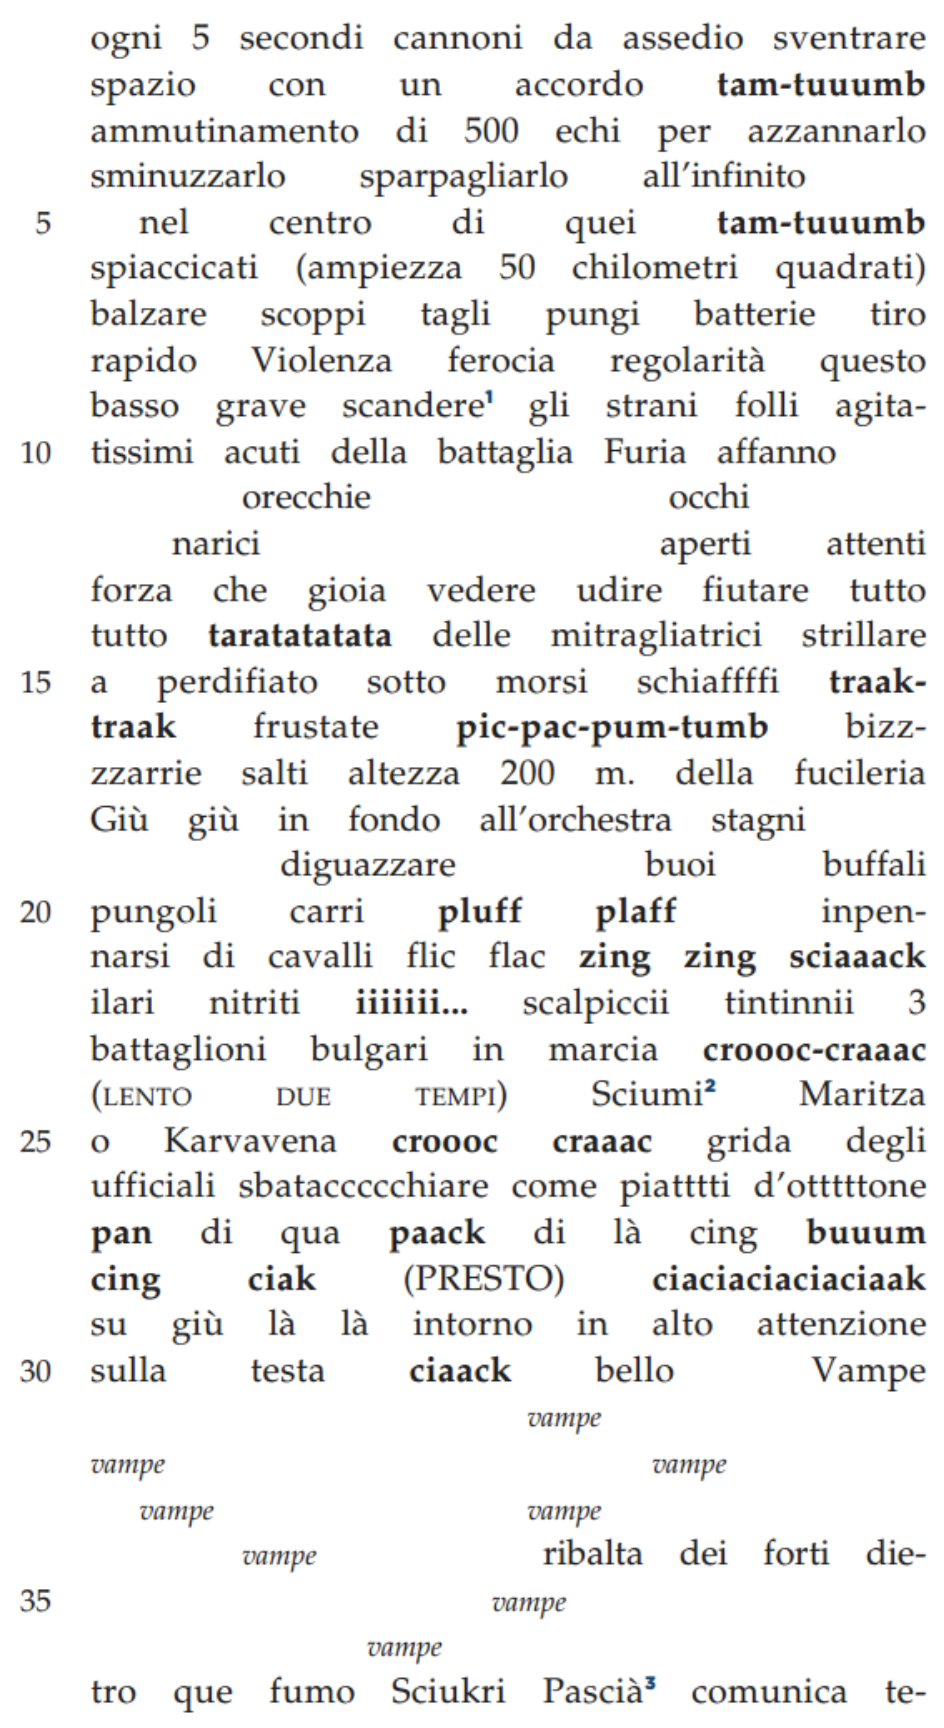
\includegraphics[width=7cm]{bombardamento1}\hfill\null
\end{minipage}

\null\hfill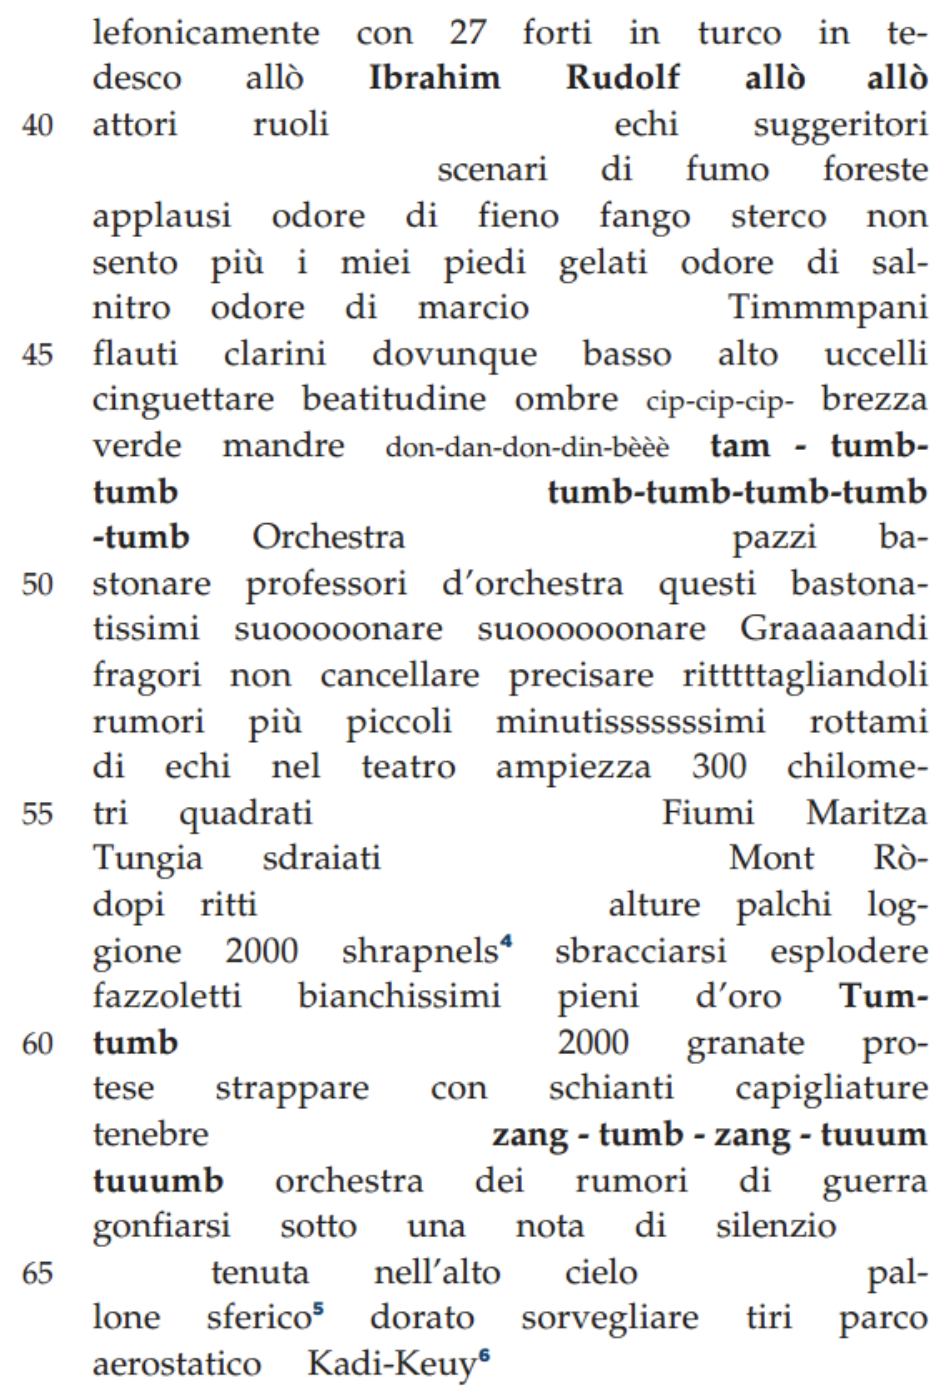
\includegraphics[width=7cm]{bombardamento2}\hfill\null
\elenco{\item \emph{p. 678}}
La poesia in generale sfrutta lo spazio in un certo modo. Non c’è niente da leggere, ma è solo sfruttato lo spazio, per rendere l’idea del bombardamento, che frattura tutto.
L’idea di sfruttare lo spazio non è nuova della poesia, perché il verso stesso sfrutta solo una parte dello spazio della pagina.

\chapter{Crepuscolarismo}

La poesia di Gozzano è di \textbf{crepuscolarismo}, un movimento che si colloca tra la fine dell’Ottocento e la prima metà del novecento.
Il crepuscolarismo si inserisce nei primissimi decenni del novecento, e Gozzano ne è l’esponente principale: è inserito nel contesto di declino della funzione della poesia e di molte forme letterarie.

Dalla fine dell’Ottocento, con una serie di cambiamenti, l’intellettuale perde la sua funzione. I vari poeti reagiscono in vari modi a questa differenza: la scapigliatura, D’Annunzio, Carducci, Pascoli.
Con il crepuscolarismo siamo contemporanei alle esperienze delle avanguardie, movimenti che cercano di rompere in modo definitivo con la tradizione.

I crepuscolari si rendono conto che c’è una rottura con il passato, e con le sue forme metriche. Mentre le avanguardie non hanno alcuna esitazione nel rompere del passato, i crepuscolari (prendendo il nome dal \textit{crepuscolo}, una zona grigia della giornata: il termine rende molto bene l’idea della poesia che hanno i poeti) prendono atto della fine di un’epoca, ma non hanno ancora qualcosa di nuovo: se la poetica dei futuristi e \textit{destruens}, le loro proposte sono significative solo di una presa di posizione, senza nulla di nuovo; i crepuscolari vivono questa sorta di fase di passaggio e di nostalgia per la poesia antica.

Il termine \textbf{crepuscolarismo} non è stato coniato successivamente. Nel 1909 Antonio Borgese, un personaggio molto importante, un critico letterario, giornalista, drammaturgo, romanziere e poeta (con un’esperienza biografica significativa: insegnante all’università che durante il fascismo dichiarò la sua non volontà di firmare fedeltà al fascismo, restando in volontario esilio negli Stati Uniti), si riferì alla poesia di questi poeti con il termine \textbf{crepuscolarismo}.

\chapter{Guido Gozzano}

Gozzano soggiornava d’estate in una villa ad Agliè. Era ammalato di tubercolosi.

Montale definirà Gozzano il “poeta dello choc”, facendo riferimento ad un procedimento usato molto spesso in Gozzano. 
Egli vive in un paradosso, consapevole del fatto che la poesia non possa più trovare nella società una funzione pubblica, la poesia si riversa in una sfera più quotidiana e intima, parlando di una realtà molto spesso prosaica: la poesia diventa prosaica, e il romanzo assume una connotazione che lo rende più simile alla poesia, concentrandosi sul frammento e sulla piccola unità da analizzare.

Gozzano cerca di provocare e di realizzare quel senso di straniamento che la poesia vive nella realtà contemporanea. La poesia vive questo senso di straniamento, in quanto è strana nel contesto in cui cerca di manifestarsi, al punto che molti poeti per sopravvivere devono lavorare in altro modo: tradurre, fare il giornalista...
Egli lo fa con degli \textbf{accostamenti arditi}. Gozzano ha una formazione classica di tutto rilievo, quindi ecco che il termine alto, Dantesco, Petrarchesco, viene calato in un contesto prosaico. Ecco da dove arriva la definizione di “poeta choc”
Molto celebre la rima di “Nietzsche” con “camicie” in una poesia di Gozzano stesso.

Le poesie sono lunghissime, con un andamento molto prosaico, con assenza di schemi metrici, di rime, e anche il linguaggio è dimesso.

Nasce a Torino, e muore molto giovane, in quanto malato di tubercolosi: tutta la sua vita sarà condizionata da questo.
Nonostante fosse nato a Torino, molto spesso si recava per dei lunghi soggiorni in Liguria, per la sua salute, o nella sua viglia ad Agliè.

Nonostante la giovane età egli produce parecchio. Le sue poesie hanno un andamento molto narrativo.

Molto spesso la sua poesia si rifà a momenti o sentimenti della sua esistenza: in parecchie si può cogliere una certa autoironia rispetto alla sua condizione di malattia.

\section{\textit{I colloqui}}

Fu la sua seconda pubblicazione, ed è una pubblicazione che va a segnare una fama abbastanza consolidata.
Il titolo ci da idea dello stile di poesia che ha Gozzano.

La poesia diventa una sorta di colloquio, di chiacchierata, tra lui e il lettore.

\subsection{T: \textit{La Signorina Felicita, ovvero la felicità}}
\elenco{\item \emph{p. 722}}

Questa poesia \textbf{racconta} una storia che il poeta decide di rievocare nel giorno dell’onomastico della fanciulla in questione: la storia tra i due, che non ha avuto compimento: la storia di un innamoramento nato in cucina, in una villa che ha perso il suo splendore, ad Agliè.
La poesia viene utilizzata anche per descrivere se stesso, come personaggio \textbf{inutile}: colui che vive in questo contesto culturale vizioso. Tutto sommato lui preferirebbe vivere di un sano lavoro manuale, che forse è la scelta migliore.

La fanciulla è semplice, non è la \textit{femme fatale} di D’Annunzio.

In particolare, in questo testo c’è una struttura di rime, un po’ atipica: le rime stesse sono rime un po’ particolari. È la poesia delle piccole cose, che anche quando tratta un tema antico come l’amore lo tratta in maniera particolare.

In occasione del 10 luglio, Santa Felicita, il poeta compone questa poesia, facendo riferimento al ricordo dell’anno precedente

\emph{Solo versi segnati}

\subsubsection{Versi 1 - 48}

\elenco{
	\item \textbf{versi 2 - 4}: c’è una analogia tra il giardino e il cuore. 
	\item \textbf{versi 4 - 5}: pensando a lei pensa anche a tutti i luoghi a lei collegati.
	\item \textbf{verso 8}: la descrizione della fanciulla, la sua lode, è completamente diversa sia alla \textit{femme fatale} di D’Annunzio che alla donna angelica provenzana: Gozzano pensa alla fanciulla, e la rivede mentre tosta il caffè.
	\item \textbf{verso 9}: i profumi descritti non sono esotici, di fiori rari, come in D’Annunzio, ma solo quello di caffè.
	\item \textbf{verso 10}: la donna cuce, e sebbene sembra che sia un tema molto antico, lei rammenda.
	\item \textbf{verso 11}: Gozzano si auto definisce “avvocato”, anche se in realtà non lo è mai diventato
	\item \textbf{verso 14}: \textit{Vill’Amarena} è la villa in cui vive la fanciulla
	\item \textbf{verso 16}: \textit{Marchesa}: è la precedente proprietaria della villa, che si è rovinata e ha dovuto dare via l’abitazione
	\item \textbf{verso 16}: \textit{dannata}: \emph{nota 4}
	\item \textbf{verso 16}: \textit{profumo tetro}: sinestesia; la tetraggine si avverte, ma non con un senso ben preciso
	\item \textbf{verso 17}: \textit{i cocci innumerevoli di vetro}: utilizzati come antifurti (\emph{nota 7}): immagine ripresa in Montale
	\item \textbf{verso 21}: \textit{cortina}: parete di granoturco
	\item \textbf{verso 22}: \textit{cimasa}: cornice di gusto barocco che decorava la casa: adesso la parete vede il granoturco riversato, messo lì a seccare: l’utilizzo della casa è molto prosaico
	\item \textbf{versi 23 - 24}: la casa è paragonata ad una dama del seicento costretta a vestirsi da contadina
	\item \textbf{verso 30}: \textit{Fiabe defunte delle sovrapposte}: \emph{nota 11}
	\item \textbf{versi 37 - 42}: \textit{che malinconia}: epifora
	\item \textbf{verso 39}: \textit{pirografia}: \emph{nota 16}
	\item \textbf{verso 41}: \textit{Otero}: \emph{nota 18}
	\item \textbf{verso 45}: la fanciulla rammenda
	\item \textbf{versi 46 - 47}: \textit{semplicità}: anafora}

\subsubsection{Versi 73 - 90}

Andando a riprendere le descrizioni evanescenti della fanciulla angelica, si può confrontare con la descrizione della fanciulla di Gozzano, che è \textit{quasi brutta}, \textit{priva di lusinga} (\textbf{verso 73}): è \textit{buona e casalinga} (\textbf{verso 75})
\elenco{
	\item \textbf{versi 79 - 80}: \textit{bocca vermiglia // così larga}: la bocca è rossa, come richiesto dalla tradizione, ma la descrizione seguente è tutto fuorché tradizionale
	\item \textbf{verso 84}: \textit{d’un azzurro di stoviglia}: è una similitudine assolutamente prosaica, novità assoluta}

La fanciulla a modo suo fa capire che è attratta dal ragazzo, e lo fa in modi semplici (\emph{note 34 e 35})

\subsubsection{Versi 91 - 95}

Il farmacista è quello che ha fatto conoscere i due

\emph{saltare da 96 a 120}

\subsubsection{Versi 120 - 162}

Inizia una sezione molto importante, in cui viene proposta l’immagine di un luogo della casa significativo: il solaio, con i suoi oggetti, metafora di tradizione e tempi passati.
Diventa simbolo della tradizione che alcuni intellettuali distruggono per poter andare oltre. Anche Gozzano ci dice che sono cose che non hanno più una collocazione nella casa, ma lui ci sta volentieri tra questi oggetti.
Questi oggetti hanno la funzione di ispirare il poeta.

Nel solaio c’è quell’atmosfera crepuscolare, un po’ buia

Si parla della Dama, chi è? È l’antica proprietaria della villa, c’è un ritratto della donna che è stato posto nel solaio, in quanto porta disgrazia. Abbiamo i due giovani che hanno fatto una passeggiata per la casa e si trovano nel solaio, la Marchesa nel ritratto ha una moda tipica della sua epoca, ci viene spiegato come la donna sia ritratta, è in un ambiente idilliaco, in una grotta artificiale, con un piede in mano.

\elenco{
	\item \textbf{riga 151}: \textit{rideva illusa}: si riferisce alla marchesa, illusa di rimanere sempre giovane
	\item \textbf{riga 153}: \textit{stirpe}: utilizza il termine che fa riferimento ai discendenti di una casata importante, che nella realtà della soffitta diventano gli oggetti (ciarpame) che sta intorno al quadro
	\item \textbf{verso 156}: \textit{caro alla mia Musa}: il ciarpame alimenta l’ispirazione del poeta
	\item \textbf{versi 161 - 162}: la fanciulla è ignorante, e chiede perché sulla testa buffa ci sia un ramo di ciliegie: la testa buffa è Torquato Tasso, incoronato con la corona d’Alloro}

\emph{saltare da 163 a 289}

\subsubsection{Versi 290 - 295}

\subsubsection{Versi 296 - 326}

Ci troviamo di fronte al gruppo di strofe estremamente importanti per definire quella che Gozzano ritiene essere la funzione del poeta: Gozzano è assolutamente consapevole del fatto che il poeta non ha più nessuna collocazione, tanto che questo gruppo di strofe si conclude con la dichiarazione “Io non voglio più essere io”

\elenco{
	\item \textbf{verso 301}: l’esser poeta fa vivere con estrema evidenza il fatto che all’interno della società non ci sia più posto per la poesia.}

Riviviamo il sentimento della scapigliatura, non ci sono più ideali a cui affidarsi, la crisi del positivismo è evidente; c’è l’assenza di prospettive: questi sono gli anni che precedono l’ingresso dell’Italia in guerra, e questa atmosfera era percepita.

\elenco{
	\item \textbf{versi 302 - 306}: \textit{Oh! [...] di vita}: il poeta dichiara di preferire una vita più rozza e grezza, rispetto alla vita contemplativa del poeta; nell’antichità si distingueva \textit{otium} da \textit{negotium}: la prima era la parte della vita relativa alla contemplazione e alle speculazione filosofica, mentre la seconda quella più pratica (a Roma la politica); c’è un confronto implicito con il fratello di Gozzano, che non ha studiato e lavora;
	\item \textbf{versi 308 - 311}: \textit{camicie} e \textit{Nietzsche}: è una rima ironica
	\item \textbf{verso 318}: \textit{miei versi tuoi}: non è solo un gioco di parole, ma la poesia è dedicata alla donna}

C’è una dichiarazione di poetica, che ci presenta il poeta come i tanti personaggi degli autori di questo periodo. Il poeta è un inetto, non è più adatto.

\chapter{Umberto Saba}

Pur collocandosi nel contesto di presa di coscienza rispetto al fatto che la tradizione poetica non è più percorribile, abbiamo un atteggiamento (quello di Saba) che si contrappone a quello visto nelle avanguardie, con una rottura netta rispetto alla tradizione.

Anche Saba rappresenta una rottura rispetto alla tradizione, ma il suo atteggiamento è quello del rinnovamento della poesia (anche grazie al suo rapporto ideale/reale con due poeti della tradizione: Leopardi e D’Annunzio)

Egli è l’ultimo poeta che si pone in un contesto di poesia che vuole concedere al lettore la comprensione diretta del testo (dopo arriverà l’ermetismo, cambiando anche i tempi, con il fascismo e la censura degli antifascisti). La poesia di Saba è ancora accessibile.

Certamente non è più rivolta a temi che spesso sono stati il pilastro della poesia (temi civili, l’amore); la poesia è più intima, tutta volta all’interiorità. 
Quando Saba parla di sé stesso uomo, si riferisce ad una situazione che vale per l’intera umanità.
Ciò nonostante non si può prescindere la sua biografia.

Saba, in una sorta di Poetica, dice che la sua poesia è facile e difficile: facile perché la struttura e lo stile sono molto facili e semplici, ma difficile perché la sua poesia si dipana come una sorta di romanzo autobiografico, e tutte le sue poesie (raccolte ne \textit{Il Canzoniere}) sono piene di rimandi.
Non possiamo estrapolare un testo e comprenderlo, ma bisogna che questo sia inserito nel contesto dell’Intera opera poetica

\section{Biografia}

Saba nasce nel 1883 (come Gozzano), a Trieste (elemento molto significativo, come per Svevo).
Trieste è città di confine, che vede il diffondersi della cultura \textit{mittele europea}.
Trieste è protagonista di molte poesie di Saba, che la vive tutta, anche i quartieri malfamati e poveri. Egli vive anche l’atmosfera del porto di Trieste, molto importante.

L’infanzia è importantissima, perché capita qualcosa che segnerà per sempre Saba: egli è strettamente collegato alla psicoanalisi, perché lui stesso starà in cura presso uno psicanalista.
Nell’infanzia di Saba è successo che il padre di Saba abbandona la moglie quando ancora Saba non è nato, poco prima della nascita. 

Il padre è un giovane italiano cattolico, e la madre invece è ebrea. Questo è importante perché si vivrà tutto il periodo delle leggi razziali.

La madre è malata e sola, e da il bambino a balia, e lo lascia a balia per tre anni, perché non si sente in grado di prendere con sé quel bambino. Il bimbo sta per tre anni a balia.
Il \textit{piccolo Berto} crede che la balia sia la madre. La balia era croata.

Saba non si chiamava così, ma si chiamava \textbf{Umberto Poli}. La sua infanzia ha avuto delle enormi conseguenze nella sua esistenza, e di questo abbiamo prova nelle sue poesie, che parlano della \textit{sepazione dalla sua tata}.
Questa, che aveva appena perso un figlio, si legò a lui come ad un figlio.

Il padre di Umberto lasciò la madre pochi mesi prima che Umberto nascesse, e la sua nascita avvenne in un contesto doloroso, di sofferenza e di rabbia.
Sua madre, non appena il figlio nasce, lo mette a balia: la donna si chiamava \textit{Sabaz} di cognome, e questo sarà lo pseudonimo con cui l'autore si chiamerà per tuta la vita: esprime chiamarmente la scelta che Umberto fece di separare il suo destino da individuo con quello della famiglia.

Ebbe un rapporto contrastato con la madre: restò a balia fino ai tre anni, quando la madre andò a riprenderlo; per lui è stato come essere strappato dalle braccia di sua madre, che lascerà un'impronta indelebile nella psicologia del bambino. Egli andò perfino in terapia per questo.

Negli anni '40 Saba scriverà un saggio in cui da indicazioni sul come leggere la sua opera, prevalentemente autobiografica.

La sua infanzia è triste: la madre era una donna triste, asciutta, che aveva dovuto sopportare da sola il peso e la fatica di allevare un figlio; vengono rievocate abitudini della madre che ci mostrano quanto i due fossero incompatibili. Saba dimostrò ben presto una propensione per la letteratura e per la poesia, e ha una passione per Leopardi. La madre gli impediva di leggere Leopardi perché diceva che alimentava il suo pessimismo: cercherà di distoglierlo in tutti i modi dalla lettura di Leopardi, e lo spingeva a leggere Parini.

Saba racconta un episodio, avvenuto quando Saba era molto giovane: egli era molto amico del figlio di \textbf{D'Annunzio} (chiamato Gabriellino), e sperava che il padre dell'amico potesse mettere una buona parola, per farsi conoscere e far pubblicare qualcuno dei suoi testi. 
Mentre si trova a casa di D'Annunzio chiede di parlare con lui: lo porta nel suo studio, e si fa raccontare ciò che stava scrivendo. Non farà più niente per lui, e Saba in una sua poesia racconta questo incontro, finendo con 
\citazione{oltre alla cortesia, niente ne ebbi}

Sposa una donna, \textbf{Lina} (citata in tante sue poesie). Dal matrimonio nasce l'unica figlia di Saba, Linuccia.
Ci sono tantissime poesie dedicate alla figlia: donnna di grande temperamento, dalla figura esile: si sposò, ma ebbe una relazione trentennale con Carlo Levi (scrittore di \textit{Cristo si è fermato a Eboli}, fu un grande pittore - ritratto e didascalia \emph{p. 166}).


Saba conosce il padre a 20, e fino ai vent'anni era considerato "l'assassino".
Saba era ebreo da parte di madre. 

Nel 1929 inizia la terapia psicoanalitica, ad opera di Eduardo Weis, un allievo diretto di Freud: era medico molto apprezzato, tanto che pur rifiutandosi di prendere la tessera del partito fascista non venne licenziato; era un personaggio particolare, che racconta come è avvenuto l'incontro con Freud. 
La psicoanalisi entra nella poesia di Saba, ma non nel modo in cui è entrata nell'opera di Svevo: Svevo in alcune conferenze aveva detto che l'opera di Freud era servita soprattutto ai romanzieri, perché aveva offerto loro degli strumenti attraverso cui analizzare la coscienza dei personaggi. Il rapporto di Saba è diverso: si rivolge alla psicoanalisi per riuscire a colmare gli abissi che ha dentro di sé, nella sua poesia si sente la psicoanalisi, si percepisce.
Saba stesso spera che la poesia abbia una funzione psicoanalitica. Egli era turbato da crisi depressive, la più grave con la morte della moglie.

Dopo il 43, a causa delle leggi razziali, dovette fuggire prima a Parigi e poi a Firenze, e grazie ad autori italiani, quali Ungaretti e Montale, riuscì a fuggire dalle persecuzioni.
Montale, firmatario del manifesto antifascista, e Ungaretti, tesserato al partito fascista: tutta la poesia di U. va in una direzione diversa, ma neppure dopo la caduta del fascismo Ungaretti rinnegherà le sue posizioni fasciste.

\section{\textit{Il canzoniere}}
\elenco{\item \emph{p. 163}}

È una raccolta di tutte le poesie di Saba, pubblicato nel 1921.
L'elemento autobiografico è fondamentale, al punto che i componimenti sono divisi in anni: le poesie sono divise in sezioni, titolate in base al periodo della vita di Saba % TODO tabella p. 163

In un saggio successivo spiegherà come leggere la sua poesia.

Saba si pone in contrasto con tutta la cultura della sua epoca, quella cultura che cercava una rottura ed un superamento delle forme tradizionali della cultura, ma anche in contrasto con tutta la poesia definita \textbf{ermetismo}, una poesia difficile di chi non può parlare.
Saba si mantiene, da un punto di vista formale, nei canoni della tradizione, con testi dalla facile comprensione.
La sua poesia descrive ambienti comuni, bassi, all'interno di forme tradizionali.

La difficoltà della sua poesia consiste nel fatto che, essendo materia autobiografica, ogni sua poesia si può comprendere solo se inserita nel giusto contesto.

Nel corso della storia, molti canzonieri contengono poesie che si bastano da sé, si esauriscono in sé stessa. La poesia di Saba invece ha bisogno della biografia, e in questo senso è "difficile".

La \textbf{nevrosi} e la \textbf{scissione dell'io}, che appare lucidamente indagata nelle sue cause profonde e nelle connessioni remote. Ecco, per intero, l'ultimo componimento, il \textit{Secondo congedo}, di preludio e fughe:
\citazione{O mio cuore dal nascere in due scisso,
quante pene durai per uno farne!
Quante rosa a nascondere un abisso}

La poesia è un'indagine psicologica che ha quasi funzione di psicoanalisi: la scissione dell'io, tanto discussa da Pirandello, viene vissuta da Saba in prima persona, sulla sua pelle. C’è una poesia, chiamata \textit{Il piccolo Berto} dove immagina di incontrare un bambino piccolissimo che gli da la mano, ed è lui stesso. Berto è il soprannome che la sua balia gli dava, immagina di incontrare questo bambino e il Saba adulto vuole delle spiegazioni, sente una scissione nella sua personalità che non riesce a conciliare e vuole sapere dal bambino l’origine dei suoi traumi. Il bambino toglie la mano inizialmente da quella dell’adulto, ma alla fine della poesia gliela ridà. La sua poesia è una costante ricerca di una conciliazione e di un senso nella sua scissione.

L'immagine delle rose è la soluzione che prospetta Saba. L'abisso rappresenta il dolore, la vita per lui è dolore, ma ci sono le rose: le rose possono essere in quantità enorme, e possono riempire l'abisso.
Le rose sono i sentimenti, l'amore, l'affetto, momenti di felicità, che possono essere gli unici elementi che possono in qualche modo colmare e riparare il dolore che è l'abisso.

Ecco allora il bambino, che si attacca al seno della balia, che trova la sua vera famiglia nella famiglia di quella, da cui verrà poi brutalmente strappato (in apertura all'ultima delle \textit{Tre poesia alla mia balia}: "Un grido / s'alza di bimbo sulle scale. E piange / anche la donna che va via. Si frange / per sempre un cuore in quel momento // Adesso / sono passati quarant'anni"); il bambino, che non ama e teme la madre, odia il padre perché la madre gli ha insegnato ad odiarlo (in \textit{Cucina economica}, il "mio povero padre ramingo, / cui malediva mia madre; un bambino / esterrefatto ascoltava"), e solo più tardi, ormai cresciuto, imparerà a conoscerlo e a sentirlo vicino, legato a lui dal "dono" della poesia (così inizia il terzo sonetto di \textit{Autobiografia}: "Mio padre è stato per me l'assassino, / fino ai vent'anni che l'ho conosciuto.)

\subsection{T: \textit{Mio padre è stato per me "l'assassino"}}
\elenco{\item \emph{p. 210}}

La forma metrica è quella tradizionale: è un \textbf{sonetto}, con le sue rime e la sua struttura formale tipica. I termini sono estremamente semplici, non solo appartenenti al linguaggio della vita quotidiana, ma anche delle strutture sintattiche che fanno riferimento al linguaggio parlato (\textit{che}, \textbf{riga 2}).

Il \textit{"l'assassino"} tra virgolette indica il fatto che sia un termine da astrarre: probabilmente era il modo con cui la madre si appellava a lui.

Saba conosce per la prima volta il padre a vent'anni.

Saba non condanna il padre, quando lo conosce capisce che è nella sua natura, è un \textit{bambino} (\textbf{riga 3}). Il padre è un uomo che vede ancora il mondo con gli occhi di un bambino, e quindi è dal lui che ha preso il suo \textit{dono} (\textbf{riga 4}), della poesia: qui è ripreso il tema del fanciullino.

\elenco{
	\item \textbf{riga 6}: \textit{in miseria}: questa è una semplice contraddizione, non ossimorica;
	\item \textbf{riga 6}: \textit{dolce e astuto}: non è un ossimoro;
	\item \textbf{righe 9-11}: qui Saba descrive i due caratteri contrapposti del padre e della madre: il padre era \textit{gaio e leggero}, due aggettivi che danno l'idea del carattere della madre; sua madre invece \textit{tutti sentiva della vita i pesi}: oltre ad esprimere a parole come fosse il carattere della madre, questo è espresso anche attraverso una inversione, faticosa: la fatica è quella della madre, che deve sopportare tutti i pesi della vita;
	\item \textbf{riga 13}: \textit{in me stesso lo intesi}: il carattere del padre giaceva dentro di lui, nascosto
	\item \textbf{riga 14}: \textit{Eran due razze in antica tenzone}: alcune interpretazioni vedono in questo verso alla semplice differenza inconciliabile tra i due genitori, mentre altre (meno probabili) vedono in quel \textit{razze} un riferimento alla diversa religione dei genitori (madre ebrea e padre cristiano)}

\subsection{T: \textit{A mia moglie}}
\elenco{\item \emph{p. 170}}

Questa poesia è in netto contrasto con il \textit{topos} della donna angelo, alla base della poesia d'amore.

La donna che descrive Saba, invece, è proprio Lina, sua moglie, e quindi non può non tenerne conto, non tenere conto della realtà quotidiana.

Non troviamo la donna angelo, la femme fatale, ma solo una donna paragonata a tanti animali; gli \textbf{animali} sono importanti per Saba, in quanto essendo così vicini allo stato di natura rappresentano un legame tra l'uomo e Dio, in quanto parte più viva del creato. Gli animali di sesso femminile ancora di più, in quanto sono accomunati con Dio dalla loro capacità di creare.
Gli animali sono più vicini a Dio dell'uomo, e rappresentano un legame

Il contesto metrico è assolutamente regolare, ma il contenuto è innovativo.

Nella poesia ci sono una serie di motivi circolari, una serie di elementi che passano dall'animale alla moglie e viceversa: molto spesso viene descritto l'animale e la moglie viene accomunata perché le somiglia, ma il confronto va anche nella direzione opposta.

Vengono presi in considerazione animali pacifici

Un gioco che si realizza in tutta la poesia: un continuo scambio tra la donna (esattamente sua moglie, ma anche simbolo di tutte le donne) e le caratteristiche degli animali.

\elenco{
	\item \textbf{verso 24}: \textit{soavi e tristi}: è reso armonico, nonostante il tono quasi ossimorico
	\item \textbf{versi 25-26}: la giovenca gravica allude alla tematica della donna madre, importante perché associa la donna a Dio; gli animali di per sé sono più vicini a Dio degli uomini, e in particolare gli animali femmina
	\item \textbf{versi 29-30}: gesto affettuoso delle mucche quando le si accarezzano
	\item \textbf{versi 31-33}: il verso e il lamento dell'animale è un motivo importante: va a definire il lamento e il verso dell'animale come una sorta di linguaggio universale: è come se alcuni sentimenti avessero un linguaggio universale, per cui c'è una sorta di fratellanza con gli animali; dolore e amore hanno un unico linguaggio (come il pianto di un bambino, uguale in tutti i paesi del mondo); questo motivo sarà approfondito nella poesia \textit{La capra}}

Saba definisce questa una \textbf{poesia da bambino}: vista con gli occhi di un adulto può sembrare banale e ridicola, ma che se letta con gli occhi del bambino comunica sentimenti, valori e temi importanti

Saba in questa poesia inserisce tutti animali mansueti.

\elenco{
	\item \textbf{verso 52}: la gelosia è un sentimento positivo (di diverso avviso rispetto a Pirandello)
	\item \textbf{versi 53-69}: altra immagine legata alla maternità: la coniglia prima di partorire si stacca il pelo e fa un nido per i suoi piccoli; scelto un animale mansueto e \textit{femmina}}

Gli ultimi tre animali sono la rondine, la formica e l'ape: non è specificato il fatto che siano le femmine, ma le qualità che va a descrivere sono prevalentemente femminili

La rondine è presa ad esempio per la sua organizzazione: ma la qualità che la moglie possiede è la leggerezza e la gaiezza.

\elenco{
	\item \textbf{verso 79}: \textit{alla campagna}: omaggio al vago e indefinito Leopardiano}

La chiusa è circolare, ed è l'interpretazione di questa poesia: la sua sposa paragonata a questi animali più vicini a Dio.
Nella chiusa di questa poesia abbiamo la tematica del \textbf{panteismo}, ripreso poi nella capra: è un sentimento religioso per il quale Saba vede una sorta di riflesso di Dio in tutte le creature.

\subsection{T: \textit{La capra}}

\elenco{\item \emph{p. 174}}

È una poesia del 1909; il poeta immagina un colloquio con una capra.

Ci sono degli enjambement molto significativi

\elenco{
	\item \textbf{versi 5-6}: il messaggio di dolore è universale, e può essere condiviso attraverso altri messaggi; l'enjambement mette in evidenza il dolore fraterno
	\item \textbf{verso 7}: \textit{per celia}: per scherzo
	\item \textbf{verso 7}: \textit{eterno}: è universale, è per tutti
	\item \textbf{verso 8}: \textit{ha una voce}: il dolore ha un'unica voce per tutti}

Il poeta pensa che il belato sia di dolore, e tutto è dato da alcuni aggettivi presenti ad inizio poesia: \textit{sola}, \textit{legata}, \textit{bagnata}.
È però anche presente l'espressione \textit{sazia d'erba}, che serve a sottolineare che il lamentarsi non sia legato alla fame. Il suo dolore deve quindi essere necessariamente dettato da altro.

Dal momento che il poeta coglie il suo stesso dolore nella capra, sentendosene fratello, percepisce la presenza di Dio

\elenco{
	\item \textbf{verso 11}: \textit{viso semita}: qualcuno ci ha visto un sentimento negativo, altri di compassione: l'atteggiamento del poeta nei confronti della capra è di \textbf{simpatia} (dal latino \textit{patior}, ovvero soffrire insieme); la poesia è del 1909, ed è chiaro che se si interpreta il testo alla luce di quello che sarebbe successo da lì a pochi anni potrebbe sembrare che quel "semita" abbia un significato ben preciso; in realtà è probabile che nell'abitudine del poeta di passare caratteristiche tra animali e uomini abbia scelto, partendo da un dato storico, prendere il popolo ebreo come emblema della sofferenza}

\subsection{T: \textit{Città vecchia}}
\elenco{\item \emph{p. 178}}

Questa poesia nasce sorella di una precedente: \textit{Trieste} (\emph{p. 176}), a cui è un po' complementare. Il poeta è triestino.
Il poeta in \textit{Trieste} parla della sua solitudine, e di come talvolta abbia bisogno di andare nella parte alta della città, che gli consente il raccoglimento in quanto luogo silenzioso e poco frequentato.
In \textit{Città vecchia} abbiamo la sperimentazione diretta del senso di fratellanza che il poeta vive nella parte della città dove stanno le persone più umili: il porto

\elenco{
	\item \textbf{verso 4}: \textit{e affollata è la strada}
	\item \textbf{verso 7}: \textit{detrito}: è estremamente significativo, il detrito è il rifiuto: viene espresso un sentimento realistico oggettivo negativo rispetto alla funzione dell'uomo: l'uomo è un rifiuto come le merci, oggetti e uomini considerati allo stesso modo
	\item \textbf{verso 9}: \textit{infinito}: la presenza di Dio
	\item \textbf{versi 17-19}: il sentimento di panteismo è dichiarato apertamente}

Saba è completamente avulso dal simbolismo: gli oggetti non sono lì solo a simboleggiare qualcosa, ma sono proprio \textit{quegli oggetti lì} che provocano in lui quei sentimenti, senza alludere ad altro.

\subsection{T: \textit{A mai}}
\elenco{\item ==p. 193}

\emph{provare a desumere la dichiarazione di poetica scritta in questa poesia}

\subsection{T: \textit{Tubercolosi, cancro, fascimo}}
\elenco{\item \emph{p. 199}}

\emph{leggere e provare a fare collegamenti per l'esame (terza fase)}

\chapter{Ungaretti}

\elenco{\item \emph{p. 212}}

Nasce nel 1888 ad Alessandria d'Egitto: è molto importante, perché tutti i luoghi della sua esistenza sono reinterpretati nella sua poesia.
I genitori avevano tentato la fortuna altrove, e lavoravano lì; il padre lavorava al canale di Suez, e perse la vita proprio sul lavoro.

Egli si appassionò ben presto di letteratura, e rimase in questa città fino al 1912, quando passando per l'Italia si reca a Parigi a completare i suoi studi.
Si fermerà pochi anni a Parigi, ma sono importantissimi. Ci dirà di essersi riconosciuto: a Parigi, oltre a studiare incontra tantissimi artisti, poeti, scrittori, pittori: è vicino a Picasso, De Chirico, a poeti della scuola simbolista, alle avanguardie: inizia a scrivere poesie su \textit{Lacerba}, una rivista riservata alle avanguaride; conosce Marinetti.
Qui si riconosce come poeta

Nel 1914 giunge in Italia, dove, fervente interventista, decide di partecipare alla Prima Guerra Mondiale, in trincea.
Rispetto a quello che emerge dalle poesie risulta inspiegabile questo suo fervente interventismo; il suo era un sentimento patriottico, che egli cerca di rafforzare in virtù del fatto che non aveva ancora una patria: doveva essere l'Italia, ma non vi era nato e non vi aveva vissuto.
Questa partecipazione alla guerra è un tentativo di trovare delle solide basi al sentimento di patriottismo.

L'esperienza della guerra diventa qualcosa di allucinante.
\emph{immagini p. 232-233}: queste due pitture alludono usano tecniche pittoriche diverse (nella prima espressionismo). Entrambi questi due poeti e Ungaretti vissero la guerra in maniera alienante e distruttiva, e lo espressero con le loro opere.

Nel 1921 prende la tessera del partito fascista, e nel 1924 non spende nemmeno una parola in merito al Delitto Matteotti.
Non ha nessun cedimento anche dopo la caduta del fascismo, diversamente da Pirandello, che si iscrisse al partito per ragioni economiche.
L'appartenenza non si concilia minimamente con la sua poesia. Egli aveva una grande umanità: Ungaretti, grande amico di Saba, lo ha aiutato quando Saba doveva nascondersi a causa delle leggi raziali. Resta un elemento senza una spiegazione.

Nel 1936 Ungaretti si trova in Brasile, dove assume la docenza di lettere all'università San Paolo. Vive lì per alcuni anni, per ritornare poi in Italia nel 1942, assumento la cattedra di lettere all'università di Roma (grazie all'influenza di Mussolini).
Egli era un personaggio molto importante, molto influente e molto apprezzato.

\section{\textit{Allegria}}

La raccolta \textit{L'allegria} nasce dall'inserimento sotto un unico titolo di due precedenti raccolte: \textit{Il porto sepolto} e \textit{Allegria di Naufragi}. Alla fine della sua vita Ungaretti raccoglie tutta la sua opera in un testo intitolato \textit{Vita di un uomo}: è significativo dell'importanza che assume l'esperienza biografica con quella poetia

La scelta del titolo della raccolta \textit{Il porto sepolto}:
\citazione{\emph{p. 219}: citazione di Ungaretti}

La poesia può penetrare fin nell'abisso e riportare a galla qualcosa: non per mezzo di un discorso piano ed oggettivo, ma per mezzo della parola poetica.
La parola diventa parola dello spazio: la parola non spiega, ma evoca, rappresenta una folgorazione, in grado di aprire immagini e significati: questa è la \textbf{parola che illumina}

La figura retorica più amata da Ungaretti è l'analogia.
\citazione{citazione \emph{p. 217}}

La poesia di Ungaretti manca ormai dei fili, ovvero di una sintassi piana, discorsiva: le parole sono sole, circondate dal vuoto della pagina, si stagliano prepotentemente senza fili e senza legami sintattici: si caricano di un significato enorme

La raccolta \textit{L'allegria} nasce dall'inserimento sotto un unico titolo di due precedenti raccolte: \textit{Il porto sepolto} e \textit{Allegria di Naufragi}. Porto sepolto sotto il mare alludue alla profondità a cui riesce a giungere il poeta. Allegria di naufragi un po' ossimorica,

I caratteri della poesia di questa prima raccolta sono quelli più emblematici dell'arte di Ungaretti:

\elenco{
	\item una poesia in cui abbiamo una disarticolazione della sintassi, che allude alla mancanza di una qualsiasi realtà organica e definibile, ad un contesto disarticolati;
	\item abbiamo una mancanza di un qualsiasi elemento descrittivo
	\item la parola si carica di significato attraverso analogia.}

I testi di Ungaretti sono spesso brevissimi, e le parole si stagliano fisicamente su un foglio biacno, che carica le poche parole presenti di un grandissimo significato.
La struttura grafica della poesia è fondamentale per la poesia stessa. La praola si carica di significato.

L'analogia è figura significante, carica di tantissimo significato la parola: utilizza degli accostamenti rapidi e piuttosto inusuali; non ci sono i fili che collegano in modo logico o quantomeno istintivo questi elementi; questo è significativo di quella disarticolazione di prima.

Questa viene definita \textbf{poesia pura}, epurata, sciolta dal contesto: anche dal contesto storico; nonostante ci siano riferimenti storici, la poesia va al di là del dato oggettivo e del dato particolare: chi è in guerra non è necessariamente in quella guerra e in quel luogo; è un concetto che riguarda l'intera umanità. 

Nella seconda raccolta, \textit{Sentimento del tempo}, è evidente che Ungaretti recupera, a livello di forma metrica, quelle strutture più tipiche e piane della poesia italiana; guarda a quei modelli più classici, come Leopardi, nonstante le tematiche restino autobiografiche.

È significativa anche la raccolta \textit{Il dolore}, del 1947. Questa raccolta è estremamente intima, perché ha al centro, come tematiche dominanti, un dolore personale: nel '37 e nel '38 Ungaretti subisce due lutti pesantissimi: il fratello a cui era legatissimo e il figlio di 9 anni.
Passano 10 anni prima che Ungaretti riesca a metabolizzare questo dolore e di avere il coraggio di esprimerlo attraverso la poesia.

Ungaretti raccoglie prima della morte tutta la sua produzione in una raccolta che si intitola \textit{Vita di un uomo}, dove è evidente quanto l'elemento autobiografico sia importante.

\subsection{T: \textit{Porto Sepolto}}
\elenco{\item \emph{p. 227}}

È il titolo della prima raccolta del 16, che poi confluisce in \textit{Allegria}. È una poesia che allude alla funzione del poeta.

Viene un po' in mente Dante, con quel \textit{nulla di enesauribile segreto}: il tema dell'ineffabile per Dio. Qui il ragionamento è analogo, che però allude all'esperienza del poeta che è riuscito nel profondo a cogliere una verità.

Il mistero della vita dell'uomo non può essere scritto in forma piana, si può cogliere un barlume, che può essere espresso solo per mezzo della parola illuminata della poesia.

Di qui a breve nascerà l'ermetismo, e i poeti di questa corrente guardano ad Ungaretti come al loro maestro.
Quest'ermetismo allude all'impossibilità del contesto storico di esprimere chiaramente ciò che si vuole. Qui vediamo il barlume di questo concetto di impossibilità di esprimere in forma scritta.

\emph{Questa poesia non è in programma}

\subsection{T: \textit{Fratelli}}
\elenco{\item \emph{p. 228}}

Il contesto è quello della guerra, ci sono giovani che si incontrano: lo stile è nominale, asciutto, ma la prima domanda della poesia allude subito ad un messaggio di fratellanza.

Questi giovani uccidono perché si trovano in un contesto piuttosto che in un altro, da una parta piuttosto che dall'altra; si incontrano, e sono persone innanzitutto.

Quel \textit{tremante} fa riferimento alla paura, forse alla speranza; la \textit{foglia appena nata} è l'inizio di un sentimento, di fratellanza reciproca.

\emph{Questa poesia non è in programma}

\subsection{T: \textit{Veglia}}
\elenco{\item \emph{p. 230}}

Sembra che questa poesia e il dipinto di p. 232 siano la stessa cosa.

Non c'è punteggiatura: la sintassi è disarticolata in questo senso, come è disarticolata l'immagine del morto. Sembra quasi la didascalia del dipinto di p. 232.

\emph{Questa poesia non è in programma}

\subsection{T: \textit{I fiumi}}
\elenco{\item \emph{p. 238}}

Fa sempre parte de \textit{L'allegria}, ma è una poesia più distesa.

I fiumi sono i quattro fiumi presentati nella poesia: sono l'Isonzo, il Serchio, il Nilo e la Senna. Sono i quattro fiumi della vita di Ungaretti.
Ungaretti è sul carso, e una notta si immerge nel fiume Isonzo. L'acqua ha una valenza simbolica, di purificazione, e in questo momento di quasi estasi, dalla presenza di questo fiume nasce il ricordo degli altri tre che hanno segnato la sua vita.
Il Serchio è un fiume toscano che gli ricorda le sue origini. La Senna è il fiume parigino, che gli torna in mente per via del periodo di studi a Parigi; la Senna quindi è simbolo della sua personalità poetica. Il Nilo è il fiume della sua infanzia.

Per quanto la forma e la sintassi sia più distesa abbiamo dei versi liberi, e dei termini fortemente carichi di significato.

\elenco{
	\item \textbf{v. 1}: \textit{Mi}: da l'impressione di una poesia fortemente autobiografica
	\item \textbf{v. 1}: \textit{mutilato}: dai colpi delle armi
	\item \textbf{v. 2}: \textit{dolina}: avvallamento, una sorta di culla per il poeta: viene paragonato ad un circo prima o dopo l'inizio dello spettacolo, quando c'è quel senso quasi di solitudine
	\item \textbf{v. 9}: \textit{disteso}: significa immerso
	\item \textbf{v. 10}: \textit{urna} è molto significativo, perché è l'oggetto in cui si conservano i morti
	\item \textbf{v. 14}: \textit{mi levigava}: azione corrosiva dell'acqua; il sasso è simbolo di morte e aridità; lui si sente ridotto come a qualcosa priva di vita
	\item \textbf{v. 17}: \textit{le mie quatt'ossa}: termine fortemente allusivo, residuo di un corpo umano; paragonato al sasso per assonanza
	\item \textbf{vv. 19-20}: \textit{l'acrobata sull'acqua} da il senso di fragilità: è una acrobazia stare sul campo di battaglia
	\item \textbf{v. 29}: \textit{mi sono riconosciuto}: ho capito di essere
	\item \textbf{v. 30}: \textit{docile fibra}: vuol dire "che si piega"; l'io lirico si sente una fibra che si piega, e sente di appartenere all'universo
	\item \textbf{v. 36}: \textit{quelle occulte mani}: sono quelle della natura; esperienza panica}

Passa in rassegna i suoi fiumi, che corrispondono alle epoche della sua vita.

\elenco{
	\item \textbf{v. 55}: \textit{inconsapevolezza}: l'inconsapevolezza è caratteristica dell'infanzia
	\item \textbf{v. 58}: \textit{torbido}: sono le contrastanti esperienze culturali con cui è venuto a contatto
	\item \textbf{v. 63}: \textit{nostalgia} è un termine molto evocativo. I \textit{nostoi} sono i poemi del ritorno (di cui fa parte anche l'Odissea); sentimento di dolore dovuto al distacco da qualcosa
	\item \textbf{vv. 68-69}: \textit{corolla di tenebre}: la corolla è quella dei fiori, immagine positiva, ma ci sono anche le tenebre}

\subsection{T: \textit{San Martino del Carso}}
\elenco{\item \emph{p. 242}}

È una poesia in cui l'immagine dell'analogia si esprime al massimo grado. Analogia tra il cuore e il paese. Sono distantissimi questi due concetti. Il poeta negli ultimi due versi lo esprime in modo esplicito.
Questa analogia si gioca sul fatto che il paese sia bombardato, distrutto dalle armi e dalla morte, e il cuore del poeta è come un cimitero: la distruzione è dovuta ai lutti e alle morti; anche il suo cuore si presenta con l'immagine di qualcosa fatto a brandelli.

\elenco{\item Anafora: \textit{di}, all'inizio di ogni riga evidenza della struttura ordinata, parallelismi nella poesia.\item \textbf{v. 4}, \textit{Brandello}: termine che normalmente si riferisce a pezzi di carne, qui è trasferito sul muro.}

L’analogia è improvvisa, perché prima è solo allusa, attraverso parallelismi.

Nella prima strofa c'è l'immagine del paese, nella seconda l'immagine del cuore, e nella terza l'analogia cuore-paese

\subsection{T: \textit{Mattina}}\elenco{\item \emph{p. 246}}

È il filo rosso di questa raccolta. È piccola nel foglio bianco.

\subsection{T: \textit{Soldati}}\elenco{\item \emph{p. 248}}

Uno degli elementi fondamentali della poesia è proprio in quel \textit{si sta}: è anonimo, impersonale; le foglie sono indistinguibili l'una dall'altra, come i soldati, che sono anonimi.

\subsubsection{T: \textit{es. 5}}
\elenco{\item \emph{p. 229} - non in programma}

È una poesia di Saba, che riporta in poesia le parole di una lettera di un suo compagno giovane morto in guerra.

\chapter{Cesare Pavese}

La figura poetica di Pavese è fortemente emblematica del suo tempo e della crisi che gli eventi storici hanno prodotto. Alcuni motivi fondamentali sono
\elenco{\item infanzia\item mito\item esperienza della casa editrice Einaudi\item rapporto con la letteratura americana\item suicidio\item rapporto con le donne}

Il 27 agosto del 1950, dopo pochissimi giorni dal ritiro del premio strega per \textit{La bella estate} (che comprende altri tre testi) Cesare Pavese si suicida, in una stanza d'albergo; qualche giorno prima di morire, in un diario intitolato \textit{Il mestiere di Vivere}, annota queste parole, alla vigilia della partenza per ritirare il premio strega:

\citazione{\textit{22 giugno}\\
Domattina, parto per Roma. Quante volte dirò ancora questa parola?\\\
È una beatitudine. Indubbio. Ma quante volte la godrò ancora? E poi?\\
Questo viaggio ha l'aria di essere per essere il mio massimo trionfo. Premio mondano, D. che mi parlerà - tutto il dolce senza l'amaro. E poi? e poi? [...]}

Quella "D." sta per Doris, la sorella di Conni, attrice di cui è innamorato. Pavese si innamora di Conni, hanno una storia, ma poi lei riparte per gli Stati Uniti e lo abbandona.
Quando ritira il premio strega ci sarà Doris accanto a lui

\citazione{\textit{14 luglio}\\
Tornato da Roma, da un pezzo. A Roma, apoteosi. E con questo?\\
Ci siamo. Tutto crolla. L'ultima dolcezza l'ho avuta da D. non da lei.}

\citazione{\textit{18 agosto}\\
La cosa pià segretamente temuta accade sempre.\\
Scrivo: o Tu, abbi pietà. E poi?

\vspace{1em}
\noindent Basta un po' di coraggio.

\vspace{1em}
\noindent Più il dolore è determinato e preciso, più l'istinto di vita si dibatte, e cade l'idea del suicidio.

\vspace{1em}
\noindent Sembrava facile, a pensarci. Eppure donnette l'hanno fatto. Ci vuole umiltà, non orgoglio.

\vspace{1em}
\noindent Tutto questo fa schifo.\\
Non parole. Un gesto. Non scriverò più}

Dopo dieci giorni si uccide in una camera dell'Hotel Roma, a Torino, in piazza Carlo Felice. Lascia una nota sulla copertina del suo libro, in cui è scritto
\citazione{Perdono tutti e a tutti chiedo perdono. Va bene? Non fate troppi pettegolezzi}

Il suo suicidio è un suicidio annunciato; nel suo diario già da molto tempo compare questo termine, ed è l'epilogo di una esistenza travagliata che inizia nel 1908. Nasce a Santo Stefano Belbo, in provincia di Cuneo.
Resta presto orfano di padre, e riceve una educazione impartita dalla madre; il rapporto con la madre è complesso; la madre è energica, cresce da sola dei figli, e soprattutto è dura, non riesce a capire la fragilità psicologica del figlio: questo causerà una insicurezza e di paura del mondo. 
Uno studioso, Fernandez, vede nel personaggio due personalità: fece le scuole medie a Torino, in una scuola dove studiava l'alta borghesia, dove ha una grandissima difficoltà di inserimento, passando il tempo a vageggiare il mondo contadino lontano, in cui comunque si sentiva a disagio.
Egli vive una sorta di inettitudine nel mondo che lo circonda.

Frequenta il Liceo Massimo D'Azeglio, a Torino. Qui ha come professore un certo Monti, che riunisce intorno a sé un gruppo di giovani intellettuali, uniti dall'odio per il fascismo. Questo professore lascerà un segno indelebile sui giovani, che saranno i futuri fondatori della Casa Editrice Einaudi.

Inizia la facoltà di lettere, dove inizia la passione per la letteratura americana; famosa è la sua traduzione del \textit{Moby Dick} di Melville. La letteratura americana avrà un'influenza grandissima in Pavese.
Sarà lui a introdurre nella cultura italiana la letteratura americana, con le sue traduzioni.

Inizia a lavorare nella casa editrice Einaudi, fino al 1935, quando la casa editrice viene chiusa a causa del fascismo.

\section{\textit{Il mestiere di vivere}}

Come documento umano questo testo rende superfluo ogni commento. Ma \textit{Il mestiere di vivere} è anche uno dei più alti esempi di letteratura autobiografica del Novecento, e come tale va considerato. Già normalmente tesa e serrata, la scrittura si fa sempre più rotta e concentrata, contraendo l'andamento analitico e riflessivo in toni sentenziosi ed epigrafici. Di fronte all'ineludibilità dell'evento, il pensiero si riduce a frammenti, che sembrano arrestarsi alle soglie di quel silenzio tante volte indicato, da Pavese, come un approdo riso lutivo della vita e della stessa letteratura.

Il motivo di fondo - cui lo scrittore allude oramai con una sorta di estraneità disincantata - è costituito dalla delusione amorosa, che viene a ribadire la convinzione di un'impotenza e di un'inutilità esistenziali incapaci di trovare conforto nei successi del presente o nelle speranze del futuro. Non resta, come motivo di consolazione, che uno scarno bilancio del passato: «La mia parte pubblica l'ho fatta - ciò che potevo. Ho lavorato, ho dato poesia agli uomini, ho condiviso le pene di molti». E della poesia resta ancora qualche eco o suggestione, ad animare l'accorata amarezza delle notazioni diaristiche. Alcune espressioni («È lei, la venuta dal mare», «Sono onde di questo mare», «Anche tu sei la primavera») rinviano infatti al gioco metaforico delle ultime raccolte di versi (vedi \textit{Terra rossa terra nera}, \textbf{v. 2}: «tu vieni dal mare»; \textit{Hai viso di pietra scolpita}, \textbf{v. 3}: «sei venuta dal mare»; \textit{You, wind of March}, \textbf{v. 5}: «Sangue di primavera»; \textit{The cats will know}, \textbf{v. 21}: «viso di primavera»).

\section{Casa Editrice Einaudi}

Intorno a questa casa editrice nacquero e lavorarono alcuni tra i letterati più importanti della letteratura italiana. Fondata nel 1933 da quegli allievi del Liceo Classico D'Azeglio, che avevano avuto come professore Monti.
Sono tantissimi i letterati che ruotano intorno a questa causa editrice. Il fondatore fu Giulio Einaudi, ma di fatto il primo direttore fu Leone Ginzburg, marito di Natalia Ginzburg (nata Levi).

Aveva due sedi, una a Torino e una a Roma. Il logo di questa casa editrice è costituita da uno struzzo, ed è mutato nel tempo. È uno struzzo a testa alta che non si nasconde dentro la sabbia; una delle versioni di questo logo era stata donata da Picasso.
Nel 2000 abbiamo l'ultima versione del logo, disegnata per la fiera di Francoforte: è uno struzzo stilizzato che ne contiene all'interno un'altro (il disegno originario). L'innovazione quindi non è disgiunta dalla tradizione

\vspace{1em}

Inizia a lavorare nella casa editrice, e nel 1935, sebbene fosse iscritto al partito Fascista (cosa necessaria per insegnare), vengono trovate nel suo appartamento delle lettere compromettenti: viene arrestato e mandato al confino in Calabria; esperienza traumatica; da qui inizia a tenere un Diario, che venne poi pubblicato postumo: \textit{Il mestiere di vivere}

Pavese scrive sia raccolti di poesie che testi in prosa. I motivi della produzione sono i medesimi. Tra le raccolte di poesie più importanti abbiamo \textit{Lavorare Stanca}.

I motivi sono
\elenco{\item il rapporto tra città e campagna\item infanzia\item maturità\item impegno: }

Il motivo dell'impegno è alla base de \textit{La casa in collina}, che riflette l'esperienza di Pavese.

L'8 settembre del 1943 c'è l'armistizio, Pavese si trova a Roma per Einaudi, e tornato a Torino non trova più molti suoi amici, che si sono impegnati nella lotta partigiana; questo è un momento fondamentale, in quanto egli non ha il coraggio di seguire l'esempio di questi suoi amici, e si rifugia a Serralunga, a Crea. Di questa indecisione c'è traccia nel romanzo \textit{La casa in collina}, che racconta la storia di un giovane che entra in contatto con un gruppo di partigiani.
Questo motivo lascia delle tracce indelebili nella sua personalità, un periodo di crisi e di vergogna.

Si iscrive al partito comunista, e si dedica all'attività politica: gli sembrava un modo per intervenire attivamente nella storia; ebe un rapporto problematico con il partito, e visse anche in questo momento un grande disagio.

Nel 1950 abbiamo la sua morte; nel suo diario la parola "suicidio" compare molto frequentemente. Ci furono anche difficili rapporti sentimentali, che probabilmente acuirono il disagio dell'autore.

L'esperienza artistica di Pavese è contemporanea a quella del Neoclassicismo, ma di fatto Pavese anche quando fa riferimento alla realtà storica contemporanea cerca di coglierne i simboli di una condizione esistenziale.
Ci sono riferimenti diretti al contesto, ma assumono questo significato simbolico. 

Un elemento fondamentale della sua poetica è il rapporto con il mito. Questo motivo divenne importantissimo, al punto tale che grazie ai suoi studi sul mito e sull'etnologia, che è lo studio comparativo delle diverse culture umane, diede vita all'interno della Casa Editrice Einaudi, della collana viola, che si dedicava agli studi religiosi, etnologici e psicologici.
Questo interesse nasce nel momento in cui si rifugia nel santuario di Crea, un luogo mitico, perché secondo lui è avvenuta la rivelazione del divino.

Ci sono diversi luoghi mitici per Pavese: il più importante è sicuramente la collina, che diventa l'emblema dell'infanzia, e tutto comincia da lì.

\textit{La luna e i falò} è un romanzo molto importante, si presenta il mito giovanile dell'America.
La luna, che è parte del titolo, scandisce i ritmi della vita contadina, e i falò sono quelli accesi dai contadini di sera durante le feste. Sono i residui di una realtà arcaica, legata ai miti della terra.
A questi falò dell'infanzia si contrappongono altri falò, che sono quelli della maturità, portatori di disgrazia, che rappresentano la caduta delle illusioni.
Questo sarà l'ultimo libro che scrive.

\section{\textit{La casa in collina}}

Durante la guerra Corrado, insegnante di scuola media, si è rifugiato sulla collina torinese per sfuggire ai bombardamenti. Qui vive presso una famiglia composta da due donne (la madre e una figlia, Elvira, «zitella quarantenne»), che lo proteggono con le loro assidue premure. Una specie di ansia interiore, tuttavia, lo spinge a conoscere altre persone che si riuniscono in una vecchia osteria. Presso costoro, che discutono di politica e di opposizione al fascismo, ritrova Cate, la donna che aveva amato un tempo e che aveva poi abbandonato per il desiderio di evitare ogni forma di responsabilità e di isolarsi nel suo individualistico egoismo. L'incontro pone al protagonista una serie di inquietanti interrogativi. In primo luogo Corrado avverte la necessità di un impegno e di una partecipazione politica, alla quale non sa tuttavia risolversi. Il problema della famiglia inoltre, come dovere morale e sociale, viene avvertito adesso con urgente immediatezza, dal momento che Cate ha un figlio, Dino, del quale Corrado sospetta di essere padre (ma il dubbio non verrà sciolto neppure alla fine del romanzo). I mesi che seguono l'armistizio dell'8 settembre 1943 trascorrono in una situazione di calma angosciosa e di paura. Un mattino, alla fine, l'osteria è perquisita dai tedeschi; Cate e gli amici vengono catturati. Corrado, che osserva di nascosto lo svolgersi di questi avvenimenti, teme di essere anch'egli compromesso e decide di allontanarsi dalla città. Inizia la fuga del protagonista, che verrà più tardi raggiunto da Dino. Si ripropone così il rapporto essenziale fra questi due personaggi, che prelude tuttavia alla loro definitiva separazione: mentre Dino si allontana per recarsi a combattere con i partigiani, Corrado, ormai solo, decide di tornare al paese d'origine, nelle Langhe. Ma il ritorno alla casa natale, dopo aver in contrato ovunque immagini di desolazione e di morte, non muta la precarietà della sua condizione esistenziale.

\section{La poesia}

\subsection{\textit{Lavorare stanca}: la «poesia-racconto»}

Fin dal primo manifestarsi dei suoi interessi letterari, come si è visto nella scheda biografica, Pavese sembra voler percorrere i sentieri meno battuti, sia per un gusto giovanile di anticonformistica provocazione, sia nel difficile tentativo - portato avanti sino all'ultimo con sofferta coerenza - di adeguare le sue capacità espressive all'urgenza delle sollecitazioni interiori. Questo sforzo è evidente non solo nella scelta degli autori americani da tradurre, ma anche nella ricerca poetica che condurrà, nel 1936, alla pubblicazione di \textit{Lavorare stanca}, una raccolta che occupa una posizione del tutto originale nel panorama della lirica contemporanea, in netto contrasto con la tendenza dell'Ermetismo dominante. Spiegando la genesi del componimento che apre il volume, \textit{I mari del Sud}, Pavese dichiara, nello scritto \textit{Il mestiere di poeta}, di aver concepito ogni poesia come un racconto, «chiaro e pacato», dal momento che sentiva «di aver molto da dire e di non doversi fermare a una ragione musicale nei suoi versi, ma soddisfarne altresì una logica». Di qui il tentativo di costruire un particolare tipo di «poesia-racconto», che, rifiutando ogni chiusura all'interno dell'io, si apra verso l'esterno, stabilendo un più ampio rapporto di comunicazione con i lettori. L'impianto narrativo di questa poesia (che presuppone quasi una lettura pubblica, ad alta voce) si basa su un «verso lungo», superiore come misura all'endecasillabo, che, richiamandosi addirittura alle forme epiche della letteratura delle origini, si propone di attribuire un'autonoma consistenza alle immagini-racconto.

\subsection{Antitesi e costanti tematiche}

Se la novità di \textit{Lavorare stanca} è costituita essenzialmente dal suo sperimentalismo tecnico e metrico, occorre aggiungere che queste poesie costituiscono anche un repertorio di spunti e di temi in cui è già prefigurata, embrionalmente, l'esperienza di Pavese narratore. Una sostanziale continuità o circolarità di motivi (per le ragioni che abbiamo in precedenza indicato) lega fra loro le diverse esperienze dello scrittore, riportandole ad una matrice comune. Cominciano così a delinearsi, sin dall'esordio, le coppie opposizionali su cui Pavese strutturerà gran parte dell'opera successiva: campagna e città, collegate da una serie di passaggi e gradazioni intermedie (la collina torinese, il fiume, la periferia, con i personaggi tipizzati di un ambiente suburbano, operai e prostitute, suonatori di chitarra e frequentatori di osterie); ozio e lavoro, insieme con le varianti evasione e impegno, individualismo e socialità; infanzia e maturità (la prima intesa come momento magico e privilegiato - "mitico" - di una scoperta dei sensi e delle cose, la seconda come aspirazione a un difficile equilibrio interiore o, più spesso, come rimpianto dell'innocenza perduta, segno della colpa e del fallimento); uomo e donna, visti per lo più come antagonisti, nemici, in un contrasto che ha anch'esso evidenti motivazioni autobiografiche.

Se la città rappresenta il luogo dell'inautenticità e della solitudine, la campagna, al contrario, e la collina in particolare sembrano promettere una pienezza di manifestazioni vitali, diventando la sede dei valori perduti sotto l'incalzare di una opprimente civiltà industriale. Agivano in lui anche le suggestioni dei prediletti autori americani, come scrive in un saggio del 1931 dedicato a Sherwood Anderson: «Per Anderson, tutto il mondo moderno è un contrasto di città e di campagna, di schiettezza e di vuota finzione, di natura e di piccoli uomini. Quanto tocchi anche noi quest'idea, credo inutile dire». L'immagine delle colline e delle Langhe ritorna, nella poesia di Pavese (e nel seguito della sua opera), con una monotona e insistita evidenza, risolvendosi, per questa sua ossessiva presenza, in una costante tematica. Come parola-tema privilegiata la «collina», attraverso una fitta trama di relazioni metaforiche, rinvia a un nodo di problemi più profondi, che hanno origine in un conflitto traumatico dello scrittore. L'antitesi campagna-città, considerata come schema fondamentale, resta la più idonea per inquadrare il dissidio e la dissociazione psicologica dello scrittore. Il punto d'arrivo è sin d'ora costituito da una sofferta solitudine (nella poesia che dà il titolo alla raccolta, Pavese scrive: «Val la pena esser solo, per essere sempre più solo?»), che assume accenti più acuti nelle poesie scritte durante il confino e aggiunte nella seconda edizione, del 1943 (si ricordi in particolare \textit{Lo steddazzu} - la stella del mattino, nel dialetto calabrese, - in cui il rapporto fra l'«uomo solo» e il «mare» sottolinea l'incomunicabilità e l'inutilità della vita). Alla luce delle successive indicazioni pavesiane, le parole-tema si definiranno più chiaramente come parole-mito, attorno alle quali si organizza un sistema di significati simbolici, che rinviano a situazioni misteriose e complesse. È la conquista di quella «realtà simbolica» che avverrà soprattutto attraverso il progredire dell'esperienza narrativa.

\subsection{L'ultima fase poetica}

Nel dopoguerra Pavese torna anche alla poesia. Nelle esigue raccolte La terra e la morte (1945) e \textit{Verrà la morte e avrà i tuoi occhi} (1950), uscite postume sotto quest'ultimo titolo nel 1951, abbandona la «poesia-racconto» per recuperare l'idea tradizionale della poesia come "canto", a cui è affidato il compito di esprimere liricamente, in versi divenuti adesso molto brevi, le sofferenze dell'io e il dolore della passione amorosa. Anche il mito allora, che nella prima raccolta era presente solo episodicamente e come elemento antropologico (in un componimento come Il dio-caprone l'animale si identifica con le credenze demoniache del mondo contadino), assume un valore essenzialmente esistenziale, come simbolo della desolazione e del fallimento dello scrittore.

\section{Mito, poetica e stile}

\subsection{La riflessione sul mito}

L'opera di Pavese risulta intimamente collegata alla sua sofferta vicenda umana e intellettuale, non per un generico autobiografismo romantico, ma perché in essa affondano le radici di una ispirazione particolarmente problematica e complessa. Una posizione centrale occupa la riflessione sul mito, che lo scrittore, in maniera prima istintiva e poi sempre più consapevole, considererà via via come un elemento essenziale e integrante della sua produzione letteraria, capace di chiarirne e unificarne le componenti eterogenee. L'interesse nei suoi confronti, che nasce dalla lettura di autori classici e moderni (Nietzsche, d'Annunzio, Mann), viene approfondito dallo studio di testi specialistici (di tipo etnografico e antropologico), dando vita, nel dopoguerra, ad alcuni saggi teorici. In uno di questi, \textit{Del mito, del simbolo e d'altro}, Pavese scrive:

\citazione{ Ora, carattere, non dico della poesia, ma della fiaba mitica è la consacrazione dei luoghi unici, legati a un fatto a una gesta a un evento. A un luogo, tra tutti, si dà un significato assoluto, isolandolo nel mondo. Così sono nati i santuari. Così a ciascuno i luoghi dell'infanzia ritornano alla memoria; in essi accaddero cose che li han fatti unici e li trascelgono sul resto del mondo con questo suggello mitico.}

Con la teoria del mito Pavese fissa e definisce le sue originarie intuizioni sull'infanzia e sul paesaggio ad essa legato. L'infanzia appare come il momento privilegiato, in cui il mito viene vissuto spontaneamente e inconsapevolmente; quando ci si rende conto di ciò, l'infanzia è perduta. Non solo, ma il mondo infantile è decisivo per lo sviluppo dell'in dividuo, in quanto lo determina. In questo rapporto consiste il «destino» dell'uomo, per il quale ogni ricerca di sé comporta sempre un ritorno alle origini. Di qui l'importanza che avranno per Pavese i concetti del «rustico», del «primitivo», del «selvaggio», proiettati nella regione delle Langhe, che si popolano - in Paesi tuoi - di figure animalesche e ferine (fondamentale, in questo senso, è stato l'influsso di Giambattista Vico, che nella \textit{Scienza nuova}, del 1725, aveva paragonato la fanciullezza dell'uomo all'età della «barbarie eroica», in cui si formano i miti dell'umanità e le creazioni della fantasia poetica). La collina diventa così, per definizione, il luogo mitico e "unico"; la rappresentazione delle vicende che in essa si svolgono acquista, per lo scrittore, un valore eccezionale e a suo modo irripetibile, assumendo una più profonda dimensione simbolica.

\subsection{Il compito della poesia}

Pavese credette, in questo modo, di dare vita a un patrimonio di credenze e tradizioni comuni, risalendo alle immagini primordiali dell'umanità, a quegli "archetipi" in cui si manifesta, secondo Jung, l'inconscio collettivo. Ma attraverso la proiezione di luoghi e figure mitiche Pavese ha trascritto essenzialmente una sua ossessiva e tormentata vicenda interiore, su un piano non collettivo, ma individualistico. A questo proposito così Furio Jesi ha sintetizzato il significato dell'operazione pavesiana: «La poesia» si caratterizza per lo «sforzo di "ridurre a chiarezza" i miti. E così nella poesia compaiono i nomi delle cose, o almeno i riflessi primordiali nella mitologia di ognuno: le immagini-racconto». Potremmo dire, per precisare ulteriormente il concetto, che il mito è la materia informe, mentre la poesia (nel senso più ampio del termine, che comprende anche la narrativa) deve dargli voce, rappresentarlo attraverso la parola. Il mito è dunque l'elemento preesistente, comune e universale, ma insieme oscuro e misterioso; compito della poesia è quello di portarlo a «chiarezza», di dargli una forma e un ordine, razionalizzando l'urgere scomposto di una materia irrazionale. Di qui nasce il travaglio che accompagna l'operazione artistica, che ha per Pavese sia una funzione conoscitiva e memoriale, sia una funzione terapeutica (in un senso quasi psicoanalitico) e liberatoria.

\subsection{L'arte come «mestiere»}

Per Pavese l'arte è in primo luogo una questione di tecnica. Lo scrittore ha spesso parlato di arte come «mestiere»: «il mestiere del poeta» traduce infatti, sul piano della resa letteraria, lo stesso sforzo faticoso di imparare «il mestiere di vivere». Sottoponendosi a una rigida disciplina, Pavese allontanava le tentazioni di un romanticismo torbido e sentimentale, sottoponendo gli impulsi immediati al rigore di un preciso controllo formale. Anche per quanto riguarda la narrativa, vengono rifiutate le suggestioni romanzesche, a favore di una trama che risulta spesso debole, quasi inconsistente. Essa corrisponde a una limitata estensione dell'universo tematico, che si organizza attorno ad alcuni nuclei fondamentali, tornando con ripetuta insistenza al mondo ben definito e circoscritto della sua ispirazione. Occorre anche in questo caso risalire alla concezione del mito, come risulta dal saggio \textit{Raccontare è monotono}:

\citazione{ Senza mito - l'abbiamo già ripetuto - non si dà poesia: mancherebbe l'immersione nel gorgo dell'indistinto, che della poesia ispirata è condizione indispensabile. Noi ora non vogliamo tentare una tipologia dell'ispirazione [...] - vogliamo semplicemente ricordare che in ciascuna cultura e in ciascun individuo il mito è di sua natura monocorde, ricorrente, ossessivo. Come negli atti cultuali l'evidente monotonia non offende i credenti bensì i tiepidi, così nella poesia. Bisogna crederci, cioè non avere ancora risolto criticamente il mito ispiratore. Del resto, dire stile è dire cadenza, ritmo, ritorno ossessivo del gesto e della voce, della propria posizione entro la realtà. [...] Raccontare è sentire nella diversità del reale una cadenza significativa, una cifra irrisolta del mistero, la seduzione di una verità sempre sul punto di rivelarsi e sempre sfuggente. La monotonia è un pegno di sincerità.}

\subsection{La «realtà simbolica»}

La narrativa pavesiana non obbedisce alla legge dinamica della variazione, ma a quel la statica della ripetizione. Una volta presa coscienza della propria condizione interiore, il ritmo e lo stile serviranno per rappresentare una realtà non superficiale, ma ripercorsa attraverso «un gioco di simboli che trasfigurano le cose quotidiane e dànno loro un valore e un significato, altrimenti il mondo sarebbe ischeletrito». Pavese ha scritto anche che «il simbolo [...] è un legame fantastico che tende una trama sotto il discorso», e ha aggiunto: «Ci vuole la ricchezza d'esperienze del realismo e la profondità dei sensi del simbolismo». La ricerca di una «realtà simbolica» è stata l'obiettivo della poetica di Pavese, che riteneva di averla raggiunta solo nei grandi romanzi della maturità: \textit{La casa in collina}, \textit{Il diavolo sulle colline}, \textit{Tra donne sole} e \textit{La luna e i falò}.

Per comprendere questa nozione, si ricordi che i romanzi pavesiani si basano su una precisa situazione storica, geografica e, al limite, sociologica. I personaggi si muovono in un ambiente determinato, appartengono a una classe o a una condizione sociale, vivono in un periodo ben definito. Tuttavia l'analisi di queste componenti (personaggi, ambienti, condizioni storiche) non si esaurisce in se stessa. Dal gioco dei rapporti che si stabilisce deve scaturire una «realtà segreta, che affiora», alla quale i singoli elementi esteriori, immediatamente percepibili, rinviano in forma simbolica. In questa trama di relazioni, che strutturano in profondità il tessuto narrativo, consiste la particolare qualità del linguaggio metaforico di Pavese. L'immagine della «mammella», che ricorre con ossessiva insistenza in Paesi tuoi per indicare la «collina», si propone di cogliere la «realtà sessuale della terra», secondo una forma di rappresentazione valida non oggettivamente, ma in quanto risale a una realtà mitico-ancestrale. Ma qui il simbolo, riferendosi a un'immagine sola, è ancora troppo immediato e scoperto. La metafora, costruita su questi rapporti singoli, si limita a offrire un'immagine isolata della realtà che l'autore intende comunicare. Una più profonda «realtà simbolica» si potrà ottenere solo attraverso un ritmo narrativo capace di legare incessantemente queste due componenti, con una continuità che si ripercuota sull'intero romanzo, attribuendo alle singole parti la risonanza metaforica del tutto. In questo senso \textit{La luna e i falò} sarà da leggere come una metafora comples siva della vicenda umana dello scrittore, che constata e simboleggia il proprio fallimento, al bivio tra l'impossibile partecipazione alla storia, da un lato, e il deludente ritorno alle origini, dall'altro.

Gli aspetti formali Sul piano del linguaggio e delle strutture formali, Pavese rifiuta le costruzioni elaborate e complesse, utilizzando modi e forme tendenzialmente vicine all'elementa rità del discorso parlato (cadenze dialettali, spezzature del periodo, anacoluti, uso della paratassi, con un andamento non di rado scarno ed essenziale). Ma non si tratta certo di una presunta immediatezza. Sin da Paesi tuoi (nel tentativo di foggiarsi un nuovo e moderno strumento di comunicazione narrativa), Pavese ingloba le stesse in flessioni dialettali all'interno di una lingua attenta e calibrata, che da un lato risulta particolarmente fluida e sciolta, dall'altro tende a una misura di compostezza rigore, attribuendo alla prosa moderna una sorta di classica dignità.

\section{\textit{La luna e i falò}}

Il narratore, un trovatello cresciuto in un paese delle Langhe e soprannominato Anguilla, ritorna nei luoghi d'origine a distanza di anni, dopo essere emigrato e avere fatto fortuna in America. Riaffiorano così, nella memoria, gli anni dell'infanzia e della giovinezza, dopo che era stato accolto e allevato da una povera famiglia, nel «casotto» sulla collina di Gaminella. Ma le persone da lui conosciute sono scomparse e i luoghi stessi sembrano mutati. È rimasto solo Nuto, il compagno di un tempo, con cui vengono rivissute le vicende del passato, quando Anguilla, passato al servizio di un ricco possidente, il sor Matteo, si recava alle feste dei paesi vicini, dove Nuto suonava il clarino. La presenza dell'amico, più vecchio e posato, si era rivelata decisiva: Nuto gli aveva insegnato «molte cose», dandogli il suo sostegno e aprendogli gli occhi di fronte alle dure realtà della vita. Adesso Nuto (che rappresenta la maturità di chi non è corso dietro ai sogni, ma è rimasto fedele alle proprie radici) ha anche il compito di colmare il vuoto degli anni in cui il protagonista è rimasto lontano. Quest'ultimo viene così informato delle sventure che hanno colpito le figlie del sor Matteo, in particolare la più giovane, Santa, che è stata uccisa dai partigiani. Ma neppure il dopoguerra ha portato la pace: il rinvenimento di alcuni cadaveri, che ispira a Nuto sentimenti di pietà, offre l'occasione per rinfocolare gli odi e le divisioni di parte. Nel frattempo il protagonista ha conosciuto Cinto, un povero ragazzo sciancato, che abita adesso nel «casotto» di Gaminella ed è costretto a subire i maltrattamenti del padre, il Valino. Questi, vittima della miseria e colpito da un'improvvisa crisi di follia, dà fuoco all'abitazione; solo Cinto riesce a salvarsi, assistendo nascosto alla scena, pronto a difendersi con il coltello che gli ha regalato lo stesso protagonista, al quale non rimane altro da fare che abbandonare il paese, dopo aver affidato a Nuto l'avvenire di Cinto. Il proposito di sistemarsi definitivamente nella terra d'origine è dolorosamente fallito.

\subsection{Il significato dell'opera}

Summa dell'opera pavesiana, \textit{La luna e i falò} ne riassume le tematiche di fondo, all'insegna di una sostanziale circolarità di criteri ispiratori. Per più versi analoga è la situazione presentata dal romanzo rispetto a quella della poesia dell'esordio, \textit{I mari del Sud}: anche in quel testo lontano il motivo conduttore era rappresentato dal ritorno alle Langhe, dopo un lungo peregrinare intorno al mondo. In \textit{La luna e i falò} si riaffaccia il mito dell'America, che aveva suggestionato Pavese negli anni della giovinezza; ma le prospettive appaiono radicalmente mutate, in un più complesso articolarsi, e quasi ripiegarsi su se stessi, di questi motivi. In particolare, come vedremo, la riconquista delle proprie radici realizzata dal cugino nella poesia, risulterà adesso, per il protagonista del romanzo, impossibile.

\subsection{Il titolo e la realtà simbolica}

Più e meglio che altrove si precisa, a partire dal titolo di quest'ultimo romanzo, la nozione pavesiana di una «realtà simbolica», fondata sul mito. La presenza della «luna» accompagna, nelle sue fasi, le vicende del destino umano; più in particolare, scandisce i ritmi della vita contadina e il tempo circolare del suo calendario, con l'eterno ritorno delle stagioni.

I falò sono i fuochi accesi dai contadini, di notte, durante le feste paesane; elementi superstiti di una realtà arcaica, legata ai miti della terra e ai riti di propiziazione, hanno rappresentato, per il bambino che li osservava, un momento magico e iniziatico di scoperta della vita, di comunione con la natura e gli uomini. A questi falò si contrappongono, sul piano dei significati dell'opera, altri falò, che comportano per il protagonista la perdita delle illusioni e la decisione di abbandonare per sempre il paese. Uno di questi è rappresentato, in senso metaforico, dall'incendio appiccato dal padre di Cinto al «casotto» della Gaminella; l'altro si riferisce, invece, alla morte di Santa, il cui cadavere viene bruciato. Ne vedremo meglio, fra poco, le implicazioni; resta il fatto che ai falò dell'infanzia, elementi che contraddistinguevano la partecipazione collettiva all'atmosfera gioiosa della festa, si sostituiranno, simbolicamente, i falò della maturità, portatori di distruzione e di morte, a ribadire una solitudine e un'estraneità ineliminabili

\chapter{Eugenio Montale}

\elenco{\item \emph{p. 296-297}: guardare bene le due pagine introduttive}

Montale è un poeta estemamente originale, e quindi nel momento in cui parliamo del suo rapporto con altri poeti (modelli e punti di riferimento) bisogna tenerne conto.
Il \textbf{correlativo oggettivo} è una figura retorica che unisce Elliot e Montale.

Nel 1975 Montale vince il premio Nobel per la letteratura. Nel discorso che pronuncerà Montale si interroga sulla \textbf{funzione della poesia}.
Egli se lo chiede sin dal momento in cui inizia a scrivere, dalla prima raccolta del 1925. Tutta la sua produzione ruota attorno a questo tema.
È un punto di arrivo di questo tema. Montale arriva a dire che il poeta non può più dire nulla, può definire la sua poesia solo in negativo. Egli non dice che non si deve fare poesia, ma che la poesia definisce in negativo: i poeti possono solo dire chi \textbf{non sono} e cosa \textbf{non vogliono}. La poesia può servire a livello etico per definire ciò che non si vuole essere.

La sua prima raccolta è del 1925, a cui segue il periodo fascista, la Seconda Guerra Mondiale. Muore nel 1981. Il periodo storico è imprescindibile dalla sua \textbf{produzione}, in quanto durante il periodo fascista era onnipresente la censura.

La poesia può agire solo attraverso illuminazioni, attraverso momenti. La sua poesia nel corso del tempo diventa difficile, per pochi, ma lui non è ermetico.
Montale non giunge a delle scelte formalmente ermetiche, ma mancano i riferimenti. È necessario studiare il contesto storico e culturale, nonché la sua esperienza culturale.

\section{Biografia}

Nasce in Liguria, e il paesaggio ligure ha profondamente influenzato la sua poesia. Nasce nel 1896 a Genova, dove passa la sua infanzia, da una famiglia mediamente agiata. Viene avviato a degli studi tecnici, diventa ragioniere, però coltiva due passione: quella per il canto (prese lezioni, e pensò per un certo periodo della sua vita di orientarsi in questa direzione; era bravissimo a quanto si dice) e quella per la letteratura. La sua formazione letteraria fu da autodidatta; si avvicinò a vari intellettuali e filosofi, frequentò i poeti liguri in gioventù, e lesse D'Annunzio, Pascoli e Gozzano; studiò Leopardi, Schopenhauer.

Partecipa alla Prima Guerra Mondiale, e subito dopo si avvicina agli ambienti antifascisti. Inizia la sua frequentazione di intellettuali torinesi, tra cui Gobetti: egli impersonava i suoi stessi ideali politici e letterari, in quanto entrambi posero un netto rifiuto contro le avanguardie.
Nel 1925 firma il \textit{Manifesto dei letterati antifascisti}, e si rifiutò di aderire al partito fascista. 

Va a Firenze, dove ottiene incarichi di prestigio; divenne direttore del gabinetto letterario di Viessaux, ma nel 1938, a causa della sua manifesta non appartenenza al partito Fascista venne esonerato da questo impiego. Non sarà mai esiliato, ma nel 1938, quando escono le leggi razziali, darà accoglienza a Saba e ai suoi familiari.

La prima raccolta è \textit{Ossi di Seppia}. Continua la sua attività di Giornalista, scrive per il Corriere della Sera a Milano, e in generale gode di grandissima stima nell'ambiente letterario.
Fu lui a tradurre e a portare alla conoscenza del pubblico italiano alcuni autori stranieri, tra cui Joyce, ma anche autori italiani, come Svevo. Nella sua rivista \textit{Solaria} scrisse un inserto proprio su Svevo, che fu quello che lo fece conoscere al grande pubblico.

La moglie di Montale è Drusilla Tanzi conosciuta nel 1939 e sposata nel 1962; nelle sue poesie la moglie viene chiamata Mosca, a causa degli occhi spessissimi per la sua miopia.

Nel 1975 viene insignito del premio Nobel (come Pirandello), e nell'81 muore.

\section{\textit{Ossi di seppia}}

Gli ossi di seppia vengono attaccati alle gabbie del canarino. Sono dei residui secchi di molluschi. Sono dei residui animali, secchi.

Il primo correlativo oggettivo, forse il più emblematico della poesia di Montale, sono prorpio questi ossi di seppia.

Il \textbf{correlativo oggettivo} è tutta una serie di oggetti e situazioni, veri e materiali, che diventano l'emblema di un sentimento, di una situazione psicologica, di un dolore. Non alludono, ma sono proprio l'emblema, qualcosa di concreto. Qui abbiamo la corrispondenza tra il sentimento e un oggetto.

Gli ossi di seppia sono l'esistenza umana nella sua lotta contro la natura, una lotta che lascia gli esseri umani come un avanzo della natura, un residuo, senza vita, disseccato. L'osso di seppia rappresenta questo stato (evidente l'esempio di Leopardi) che non può essere spiegato in termini oggettivi.

Montale cerca di rifiutare il determinismo che fa sì che tutto sia preordinato oggettivamente, con dei rapporti causa effetto. Montale cerca l'anello mancante, quello che non tiene, il varco attraverso cui l'uomo possa uscire da questa situazione esistenziale. Ci sono illuminazioni qua e là, ma di fatto l'uomo non può uscire.
Ci sono delle immagini, come la muraglia, che tiene prigioniero l'uomo. Montale cerca il varco, che non si trova. Ci sono delle illuminazioni, le rose nell'abisso di Saba, momenti di rara felicità che ci sono nell'esistenza dell'essere umano; sono solo momenti.

La raccolta esce nel 1925.

\subsection{T: \textit{Spesso il male di vivere ho incontrato}}

\elenco{\item \emph{p. 315}}

Il testo risale probabilmente al 1924.

Le parole e le costruzioni sintattiche non sono difficili, ma Montale non esplicita passaggi intermedi e riferimenti. La sua poesia è difficile perché mancano i riferimenti interni.

Più oggetti veri diventano l'emblema di un sentimento. In questa poesia c'è prima il sentimento (il \textbf{male di vivere}) che gli oggetti.
\elenco{\item \textbf{v. 1}: \textit{incontrato}: l'incontro prevede la presenza di due entità fisiche: qui Montale utilizza questo verbo riferito ad un sentimento; questo verbo rende concreto un sentimento astratto\item \textbf{v. 2}: \textit{rivo strozzato che gorgoglia}: la liguria di Montale non è verdeggiante, ma è quella del periodo estivo torrido: il rivo è un piccolo corso d'acqua, quasi prosciugato; il gorgogliare è un suono sinistro, perché c'è quello \textit{strozzato}\item \textbf{vv. 3-4}: \textit{l'incartocciarsi della foglia // riarsa}: il sole di Montale è un sole che secca, che crea aridità e prosciuga\item \textbf{v. 4}: \textit{il cavallo stramazzato}: il linguaggio si abbassa}

L'unica via di fuga è l'indifferenza, non intesa come un atteggiamento di menefreghismo, ma una indifferenza stoica: bisogna essere capaci di prendere le distanze e di elevarsi da queste bassezza.
La seconda strofa contiene tre correlativi oggettivi per l'\textbf{indifferenza}:
\citazione{ Non ho conosciuto felicità al di fuori di una situazione eccezzionale concessa dalla divina indifferenza:}

\elenco{\item \textbf{v. 5}: \textit{non seppi bene}: è autobiografico, e significa che non ha conosciuto felicità\item \textbf{v. 6}: \textit{divina Indifferenza}: riferimento a Manzoni con la sua Divina Provvidenza}

L'indifferenza è l'unica via percorribile.

Le tre immagini danno un'idea concreta del sentimento dell'indifferenza:
\elenco{\item \textbf{vv. 7-8}: \textit{la statua nella sonnolena // del meriggio}: la statua è di pietra, e può godere di quello stato per cui non si sente male\item \textbf{v. 8}: \textit{la nuvola, e il falco alto levato}: sono entrambi in alto, e possono estraniarsi da questa bruttura concreta, che è il male di vivere; sono estranei alla condizione dell'uomo.}

L'unico modo per sopravvivere all'esistenz e a questa bruttura è estraniarsi, vivere l'indifferenza stoica del poeta.

\vspace{1em}

Ci sono dei motivi ricorrenti in questa raccolta: 
\elenco{\item il \textbf{correlativo oggettivo};\item la \textbf{muraglia}: rappresenta la prigione che tiene l'uomo e da cui non può uscire; è la condizione esistenziale; la muraglia imprigiona l'uomo, e l'uomo cerca di continuo di darsi una spiegazione della sua esistenza, cerca di uscire da questa muraglia (il \textbf{varco}); ci sono solo delle illuminazioni\item le \textbf{pozzanghere} e le \textbf{anguille\textbf{, che assumono il significato di correlativo oggettivo che rimandano ad altro, soprattutto il senso di }arsura} e \textbf{secchezza} che caratterizza l'esistenza dell'uomo.}

\subsection{T: \textit{I Limoni}}

\elenco{\item \emph{p. 306}}

Questa è una poesia manifesto contro l'aulicismo, impersonato da D'Annunzio e da Carducci. Vediamo la centralità degli oggetti, e quindi possiamo vedere l'influenza di Pascoli e di Gozzano.
È una presentazione oggettiva, con la presenza del correlativo oggettivo.

Il paesaggio nasce dall'esperienza dell'infanzia in Liguria.

\elenco{\item \textit{erbosi fossi}: è un enjambement: fissa l'attenzione su questi termini}

È una poesia programmatica che ci da informazioni sulla poetica di Montale, e che si interroga sulla funzione della poesia. Qui entra nel dettaglio della poetica, e prendendo le distanze da Dannunzio ci presenta il suo modo di fare poesia, in cui gli oggetti hanno una fondamentale importanza.

C'è un interlocutore, che sarà chiamato in causa più volte all'interno della poesia; abbiamo un io e un noi; ad un certo punto il poeta rinuncia ad essere una identità ben definita (un io) e diventa un "noi" che sta ad indicare tutti i poeti; è sentirsi associato ad un gruppo che non sa ben dire come stanno le cose.
La poesia può dire ciò che non si è, ma non rivelare verità.

Chiama in causa il lettore, e poi i lettori, quasi a farli partecipi di questa indecisione.

\elenco{\item \textbf{v. 1} \textit{Ascoltami}: è un chiaro riferimento a D'Annunzio. Non si può ignorare D'annunzio, però Montale lo oltrepassa, e ci dice ciò che la sua poesia nonfa\item \textbf{v. 3}: \textit{bossi ligustri o acanti}: piante utilizzate dai poeti\item \textbf{v. 4} \textit{io per me}: espressione estremamente colloquiale e sintattivcamente scorretto: abbassamento da parte di Montale rispetto al loquio usato dai poeti laureati; sta per indicare la volontà di rimanere estraneo\item \textbf{vv. 5-6}: \textit{pozzanghere mezzo seccate}: ossimoro\item \textbf{v. 8}: \textit{viuzze}: la Liguria di Montale è quella dell'entroterra\item \textbf{v. 9}: \textit{canne}: sono piante meno nobili di quelle citate all'inizio.}

I limoni rappresentano la luce e l'illuminazione; possono essere quel momento epifanico, quella illusione, quella speranza; sono correlativo oggettivo del sentimento della speranza che verrà deluso.

È una poesia particolarissima; qui si sente l'eco della \textit{Pioggia nel Pineto}, con la rievocazione delle stesse impressioni, ma i rumori sono diversi. Tutta la seconda strofa è giocata su impressioni uditive e olfattive

\elenco{\item \textbf{vv. 13-14}: \textit{sussurro dei rami amici}: è il sussurro dei limoni; il limone non è una pianta con molto fogliame, quindi non provoca un particolare sussurro; è qualcosa evocato attraverso un rumore, anche se non è proprio un rumore.\item \textbf{v. 13}: \textit{più chiaro si ascolta il sussurro}: sinestesia molto particolare, evocata in modo originale (di solito si hanno due sostantivi)\item \textbf{v.17}: \textit{dolcezza inquieta}: allude al conflitto delle passioni che ci sono dentro l'animo}

Il profumo dei limoni è l'evento epifanico. 

\elenco{\item \textbf{v. 18}: \textit{divertite}: significa separate, divise. \item \textbf{v 19}: \textit{per miracolo tace la guerra}: anastrofe}

% TODO qualcosa (me li manda noemi)

Da questo momento ci si aspetta di scoprire lo \textit{sbaglio della natura}, il \textit{punto morto del mondo}: in questi momenti di abbandono ci si aspetta di trovare il varco per oltrepassare la muraglia.

\elenco{\item \textbf{v. 24}: \textit{ultimo segreto}: la rivelazione che ci si aspetta riguardo la condizione esistenziale dell'uomo\item \textbf{vv. 30-31} Questi versi fanno riferimento al continuo tentativo da parte dell'uomo di darsi una spiegazione, di trovare un senso razionale delle cose}

Il profumo dei limoni è il correlativo oggettivo della speranza dell'uomo.

Per quanto Montale dichiari di voler abbassare il tono, ci rendiamo conto che la sua è una volontà, non l'incapacità; in questi versi abbiamo tantissime figure retoriche, abbiamo molti rapporti intertestauli con altri autori

\elenco{\item \textbf{vv. 34-35} è il momento dell'attesa epifanica, in cui ci si aspetta la rivelazione che possa svelare il varco. In quei momenti ci si aspetta di vedere la divinità in ogni presenza, ed è dalla divinità che ci si aspetta di avere una rivelazione. La nostra predisposizione d'animo ci fa vedere una divinità\item \textbf{v. 37}: l'avversativa e il cambio di paesaggio rappresentano la caduta della speranza di poter avere questa rivelazione}

Nonostante tutto nel finale abbiamo un barlume di speranza. L'illusione viene definita nei termini di qualcosa che può illuminare per un momento, sono piccoli episodi, illuminazioni temporanee.

\elenco{\item \textbf{v. 39}: \textit{cimase}: i cornicioni, li abbiamo trovati in Gozzano\item \textbf{v. 40}: \textit{la pioggia stanca la terra}\item \textbf{v. 40}: \textit{affolta}: reminescenza D'annunziana\item \textbf{v. 41}: \textit{tedio}: altra tematica ricorrente\item \textbf{v. 42}: \textit{la luce si fa avara - amara l'anima}: abbiamo un chiasmo, e in più c'è paranomasia (accostamento di due parole che si assomigliano molto ma alludono a due significati molto distanti)}

Anche cadute le illusioni c'è sempre la possibilità che da un cortile si possa vedere un albero di limoni

\subsection{T: \textit{Non chiederci la parola}}
\elenco{\item \emph{p. 310}}

La poesia è del 1923, e bisogna tenerne conto.

\elenco{\item \textbf{v. 1}: \textit{non chiederci}: La poesia inizia in negativo\item \textbf{v. 1}: \textit{-ci}: i poeti\item \textbf{v. 1}: \textit{squadri}: la realtà non ha nulla di oggettivo e nulla che possa essere definito\item \textbf{v. 3}: \textit{croco}: un fiore giallino da cui si ricava lo zafferano; è piccolo, ma il suo giallo è molto vivo; per farci capire come non può essere la poesia usa questa similitudine; la parola certa si dovrebbe manifestare in modo così evidente come succederebbe a vedere un croco in un prato polveroso (simbolo delle passioni negative dell'animo umano)\item \textbf{v. 5-8}: reminescenza leopardiana, che ne \textit{La Ginestra} parla dell'uomo sicuro di sé: quell'uomo crede di avere risposte per tutto, e Montale non si sente così\item \textbf{v. 7}: \textit{ombra}: è il simbolo degli aspetti negativi della vita\item \textbf{v. 7}: \textit{canicola}: è la calura estiva; è una metonimia, in quanto lui vuole intendere la luce del sole\item \textbf{v. 8}: \textit{muro}: ciò che imprigiona l'uomo\item \textbf{v. 9}: espressione esplicita\item \textbf{v. 10}: \textit{sì}: al massimo}

Non è possibile in un contesto storico poter dare risposte. Anche soltanto l'impossibilità di esprimersi sotto il fascimo è importante. Queste verità prescindono il contesto storico, ma questo non può essere ignorato.

\subsection{T: \textit{Meriggiare pallido e assorto}}
\elenco{\item \emph{p. 313}}

Meriggiare significa riposare all'ombra nell'ora calda. Montale usa il verbo, allinfinito, e gli infiniti rappresentano un motivo di staniamento: l'infinito è un modo indefinito, che non ha la persona.

Questa poesia attraverso le immagini di oggetti e suoni molto corporei ci comunica la vita priva di vita, perché non vi è più acqua, simbolo di vita. Abbiamo un'immagine di mare che rimanda alla secchezza.

\elenco{\item \textbf{v. 1}: \textit{pruni e gli sterpi}: citazione Dantesca, canto di Pier delle Vigne\item \textbf{v. 4}: \textit{schiocchi}: onomatopea}

Tutte le sensazioni sono espresse attraverso l'infinito.

\elenco{\item \textbf{v. 8}: \textit{biche}: mucchietti su cui corrono le formiche\item \textbf{vv. 9-10}: \textit{palpitare lontano di scaglie di mare}: l'immagine del mare è restituita con una sensazione di secchezza; il palpitare da l'idea di una vita, ma abbiamo un'immagine di secchezza; le onde, colpite dal sole, sembrano scaglie}

In questa poesia abbiamo l'esempio della sintassi spezzata, e dei suoni che rimandano a concetti di secchezza, di fragilità

\elenco{\item \textbf{v. 12}: \textit{calvi picchi}: alture prive di vegetazione\item \textbf{v. 15}: \textit{travaglio}: è preannunciato dai due termini in consonanza nelle righe precedenti}

Il correlativo oggettivo della prigionia dell'esistenza è la muraglia con i cocci di bottiglia (già vista in Gozzano). L'uomo non può uscire dalla prigione che è il mistero dell'esistenza.

\section{\textit{Le Occasioni}}

Fa parte della seconda raccolta di Montale, del 1939, che si intitola \textit{Le occasioni}: rappresenta il momento più emblematico per quanto riguarda il correlativo oggettivo. Questa raccolta potrebbe sembrare essere scritta per diverse occasioni: nel corso della storia c'è sempre stata la poesia d'occasione; in realtà questa raccolta è solo fatta di oggetti, considerata stilisticamente più difficile e di ardua comprensione: volutamente Montale tace l'occasione e tutti i riferimenti biografici che sarebbero necessari alla comprensione della poesia stessa; nella poesia resta l'oggetto, il correlativo oggettivo.

Questo allontanamento dal barlume di messaggio che la poesia potrebbe dare è dovuto al fatto che siano gli anni in cui Montale prende le distanze dal contesto politico, dalla situazione di guerra, dalla società di massa; questa esclusione si manifesta attraverso questa poesia.

È ricorrente l'immagine della \textbf{donna salvifica}, la donna angelo; effettivamente abbiamo una sorta di musa che compare più volte nella raccolta, che è Clizia; questo nome è una sorta di signal, che effettivamente farebbe riferimento ad una donna realmente conosciuta da Montale, Irma Brandeis. Questa fanciulla era una donna di grandissima cultura, una americana ebrea, che si era recata in Italia appassionata di studi danteschi; incontra Montale, e sembra che la prima impressione fu assolutamente negativa; nasce però una relazione che durerà tantissimi anni. Nel '38 lei dovrà tornare in america per le leggi raziali, ma continuerà a scrivere a Montale. Questa donna rappresenta la donna salvifica.

La donna angelo dovrebbe avere la funzione di permettere l'illusione della felicità; inutile dire che la visione di Montale è assolutamente negativa; ci sono nella prima parte della raccolta ancora degli aspetti illusori che vengono poi cancellati nella seconda parte, per lascaire posto ad un totale pessimismo

\subsection{T: \textit{La casa dei doganieri}}

\elenco{\item \emph{p. 341}}

La fanciulla a cui si fa riferimento non è Irma, ma è un'altra ancora. In questa poesia la donna non è altro che un personaggio, come Laura e Beatrice, che assumono un significato \textit{altro} rispetto ad un possibile riferimento biografico. Questa fanciulla è conosciuta da Montale in gioventù, e poi si separarono, dopo un incontro fugace; questa fanciulla muore molti anni dopo rispetto alla morte poetica che le da il poeta.

Ci sono delle reminescenze di Leopardi (\textit{A Silvia}), in quanto in questa poesia il poeta si riferisce alla fanciulla morta. C'è il tema della memoria: è un tema in cui Leopardi e Montale vanno in direzione opposta;

\elenco{\item per Leopardi il ricordo, anche di momenti negativi, è positivo, in quanto nel passato erano ancora presenti le illusioni;\item per Montale invece la memoria non è possibile, il tempo offusca il ricordo, e quindi non ha una valenza positiva.}

In questa casa dei doganieri non ci sono più riferimenti; abbiamo il correlativo oggettivo del galletto segnavento, che gira all'impazzata.

\elenco{\item \textbf{v. 1}: \textit{Tu non ricordi}: fin da subito è presente il tema della negatività della memoria\item \textbf{vv. 4-5}: \textit{sciame dei tuoi pensieri [...] irrequieto}: la donna cantata è irrequieta, con un vissuto intenso; la sua interiorità è complessa, differentemente di cosa succedeva per Beatrice e Laura}

Ci sono molti oggetti estremamente significativi; il \textit{filo} fa riferimento al filo d'Arianna, ma non è più possibile seguirlo; non c'è più nulla che ci indichi la strada; emerge la mancanza di punti di riferimento

\elenco{\item \textbf{v. 6}: \textit{libeccio}: è un vento\item \textbf{v. 6}: \textit{sferza da anni le vecchie mura}: immagine di desolazione\item \textbf{v. 7}: \textit{riso non è più lieto}: la fanciulla è morta\item \textbf{v. 8}: \textit{la bussola va impazzita}: l'ago della bussola, che segna la direzione, è un correlativo oggettivo, ma è rotto, non segna più il nord\item \textbf{v. 9}: \textit{calcolo dei dadi più non torna}: mancanza di punti di riferimento\item \textbf{v. 12}: \textit{ne tengo ancora un capo}: della matassa, lui è ancora legato alla memoria, ma questa si allontana\item \textbf{v. 13}: \textit{la banderuola}: indica la direzione del vento, ma anche lui gira senza pietà, a vuoto; da una parte indica il fatto che non ci siano più punti di riferimento (non si capisce da che parte arrivi il vento), e in più fa un movimento inutile \item \textbf{v. 16}: \textit{oscurità}: non c'è nessun punto di riferimento, il buio indica ignoranza\item \textbf{v. 18}: \textit{luce della petroliera}: immagine lontana, luce che si accende ad intermittenza; può rappresentare un barlume di saggezza, che tanto poi sparisce e non si vede più\item \textbf{v. 19}: \textit{varco}: sempre lo stesso motivo dominante; è il buco nella muraglia: il poeta, quando c'è qualche luce, si chiede se quello sia il varco\item \textbf{v. 19}: \textit{frangente}: fa riferimento all'onda che ribatte sullo scoglio}

\chapter{Primo Levi}

\citazione{ Per mia fortuna, sono stato deportato ad Auschwitz solo nel 1944, e cioè dopo che il governo tedesco, data la crescente scarsità di manodopera, aveva stabilito di allungare la vita media dei prigionieri da eliminarsi, concedendo sensibili miglioramenti nel tenore di vita e sospendendo temporaneamente le uccisioni ad arbitrio dei singoli.

Perciò questo mio libro, in fatto di particolari atroci, non aggiunge nulla a quanto è ormai noto ai lettori di tutto il mondo sull'inquietante argomento dei campi di distruzione. Esso non è stato scritto allo scopo di formulare nuovi capi di accusa; potrà piuttosto fornire documenti per uno studio pacato di alcuni aspetti dell'animo umano. A molti, individui o popoli, può accadere di ritenere, più o meno consapevolmente, che «ogni straniero è nemico». Per lo più questa convinzione giace in fondo agli animi come una infezione latente; si manifesta solo in atti saltuari e incoordinati, e non sta all'origine di un sistema di pensiero. Ma quando questo avviene, quando il dogma inespresso diventa premessa maggiore di un sillogismo, allora, al termine della catena, sta il Lager.

Esso è il prodotto di una concezione del mondo portata alle sue conseguenze con rigorosa coerenza: finché la concezione sussiste, le conseguenze ci minacciano. La storia dei campi di distruzione dovrebbe venire intesa da tutti come un sinistro segnale di pericolo.

Mi rendo conto e chiedo venia dei difetti strutturali del libro. Se non di fatto, come intenzione e come concezione esso è nato già fin dai giorni di Lager. Il bisogno di raccontare agli «altri», di fare gli «altri» partecipi, aveva assunto fra noi, prima della liberazione e dopo, il carattere di un impulso immediato e violento, tanto da rivaleggiare con gli altri bisogni elementari; il libro è stato scritto per soddisfare a questo bisogno; in primo luogo quindi a scopo di liberazione interiore. Di qui il suo carattere frammentario: i capitoli sono stati scritti non in successione logica, ma per ordine di urgenza. Il lavoro di raccordo e di fusione è stato svolto su piano, ed è posteriore.

Mi pare superfluo aggiungere che nessuno dei fatti è inventato.}

Si è suicidato, lo hanno trovato al fondo della tromba delle scale. La sua vita è stata piena di altruismo, andava nelle scuole a parlare con i bambini.

Nel 1919 nasce Primo Levi, a Torino, da una famiglia ebrea borghese. Vive la sua infanzia e la sua giovineza a Torino, studia al liceo Massimo D'Azeglio. Si appassiona alla chimica e si iscrive alla facoltà di Chimica.

Nel 1938 escono le leggi raziali, e tra queste ve ne era una che dicesse che gli ebrei non potessero fare tesi sperimentali ma solo tesi compilative; lui patì tantissimo questa esclusione. Ciò nonostante si laureò nel 1942 con il massimo dei voti e la lode. Lui stesso disse successivamente che forse la sua salvezza fu proprio legata alla chimica, perché all'interno del campo le sue conoscenze chimiche venivano impiegate, permettendogli di godere di un po' di caldo.

Se da un lato la gente di cultura era sfruttata e "privilegiata", dall'altro era svantaggiata in fatto di resistenza fisica. Va detto però che avere degli appigli culturali a cui aggrapparsi permetteva di rimanere uomini, e di ricordarsene.

\emph{Leggere il capitolo dell'ulisse di Dante di \textit{Se questo è un uomo}}

Nel 1943 Levi viene arrestato (faceva parte di una banda di partigiani) e portato ad Aushwitz: era un momento in cui i tedeschi sterminavano meno, perché avevano bisogno di molta forza lavoro.
Dopo circa un anno uscirà dal lager, e inizierà il lungo ritorno (descritto ne \textit{La Tregua}), che durò 8-9 mesi. Arrivò a Torino nel '45, e subitò iniziò la stesura di \textit{Se questo è un uomo}.
Iniziò a lavorare, e affiancò al suo lavoro come chimico altre attività: Levi fu famoso anche per le sue sculture in filo di rame. L'aspetto legato al mondo tecnico scientifico riveste una importanza molto grande in Levi.

Inoltre lavorò molto per mantenere vivo il ricordo di ciò che è stato: porta la sua esperienza nelle scuole. Parlava con gli studenti, partecipò a tantissimi incontri, al punto che alla fine di \textit{Se questo è un uomo} c'è un'intera sezione dedicata alle risposte alle domande che più gli venivano fatte nelle scuole.

\subsection{\textit{Se questo è un uomo} e le altre opere}

Il primo testo di Levi è \textit{Se questo è un uomo}, del 1946. Inizialmente Einaudi non raccolse l'invito a pubblicare il testo, non aveva colto né l'importanza né l'unicità di questo teso. Il libro si distingue dagli altri perché non è solo un resoconto dell'esperienza, ma uno studio attento del comportamento umano calato in un contesto assolutamente anormale. In questo testo Levi spiega quali sono state le ragioni per cui si è salvato: la sua conoscenza di chimica, e il fatto che si ammalò quando i tedeschi decisero di far evacuare il campo di concentramento, rimanendo nell'infermeria del campo.

Ne \textit{La Tregua} viene raccontato il viaggio di ritorno, dal momento in cui viene liberato dal campo. Questo è l'unico libro tra i tre che a tratti coglie gli aspetti di un romanzo.

Ci sono altre raccolte, come \textit{Il sistema periodico}, che è una serie di racconti estremamente strani; Levi sfocia nella fantascienza, ed ebbe delle visioni illuminanti in tal senso. È un testo interessante, divertente e molto attuale.
Ritornò sul tema dei campi di sterminio, con il testo \textit{Se non ora quando}, la storia di un gruppo di partigiani russi.
\textit{La chiave a stella} è un romanzo in cui si racconta la storia di un operaio che va in giro per il mondo a costruire ponti; c'è una grande attenzione per il lavoro, anche quello manuale.

L'ultimo testo, \textit{I sommersi e i salvati}, è l'ultimo della trilogia dedicato alla sua esperienza: è una riflessione, scritta tanti anni dopo l'esperienza del lager, sull'esperienza che continua ad essere viva in Levi. Più volte ebbe modo di confrontarsi con altri intellettuali e altri superstiti su queste tematiche. In quest'ultima opera fa quasi uno studio antropologico della natura umana, colta in un contesto particolarissimo. 
All'interno del Lager non ci sono punti di riferimento attraverso i quali ci si possa fare una ragione rispetto a quanto sta accadendo. Lui ha la volontà di capire il comporamento umana, e di mettere in luce anche gli aspetti in chiaro scuro (la zona grigia): era facile capire cosa fosse il male, ma era molto più difficile cogliere gli altri aspetti dell'individuo; ad esempio, in un contesto di questo tipo ci si aspetta di trovare solidarietà, cosa che invece non avvenne: ognuno cercava di sopravvivere, ognuno per conto proprio.

\subsection{T: \textit{Se questo è un uomo} e \textit{sommersi e salvati}}

Il terrore dei testimoni dei lager era quello di non essere creduti, e questa preoccupazione è onnipresente in Levi, tanto che la prima cosa che fa tornato a casa sarà di scrivere queste memorie.

Un fatto particolare: nei primi tempi in cui si trovava nel lager, istintivamente ogni tanto si guardava il braccio sinistro per guardare l'ora: ogni volta che lo faceva vedeva, anziché l'ora, il tatuaggio; bisognava dimenticare il proprio nome e ricordarsi il proprio numero. La paura era quella di non capire gli ordini, pronunciati in tedesco: Levi era stato fortunato, perché nei suoi studi aveva studiato un po' il tedesco. 
Il suo nome era stato cancellato.

Questo primo brano riguarda la violenza fisica; la paura per la violenza fisica fu uno degli aspetti che distoglieva da qualsiasi altra meditazione: la preoccupazione costante impediva di pensare ad altro

\citazione{ Qui ricevemmo i primi colpi: e la cosa fu cosi nuova e insensata che non provammo dolore, nel corpo né nell'anima. Soltanto uno stupore profondo: come si può percuotere un uomo senza collera?

I vagoni erano dodici, e noi seicentocinquanta; nel mio vagone eravamo quarantacinque soltanto, ma era un vagone piccolo. Ecco dunque, sotto i nostri occhi, sotto i nostri piedi, una delle famose tradotte tedesche, quelle che non ritornano, quelle di cui, fremendo e sempre un poco increduli, avevamo cosi spesso sentito narrare. Proprio cosi, punto per punto: vagoni merci, chiusi dall'esterno, e dentro uomini donne bambini, compressi senza pietà, come merce di dozzina, in viaggio verso il nulla, in viaggio all'ingiú, verso il fondo.

Questa volta dentro siamo noi.}

\citazione{ Sono stati proprio i disagi, le percosse, il freddo, la sete, che ci hanno tenuti a galla sul vuoto di una disperazione senza fondo, durante il viaggio e dopo.

Non già la volontà di vivere, né una cosciente rassegnazione: ché pochi sono gli uomini capaci di questo, e noi non eravamo che un comune campione di umanità.}

Il problema della lingua, la mancanda di comunicazione

\citazione{ Venne a un tratto lo scioglimento. La portiera fu aperta con fragore, il buio echeggiò di ordini stranieri, e di quei barbarici latrati dei tedeschi quando comandano, che sembrano dar vento a una rabbia vecchia di secoli.

Una decina di SS stavano in disparte, l'aria indifferente, piantati a gambe larghe. A un certo momento, penetrarono fra di noi, e, con voce sommessa, con visi di pietra, presero a interrogarci rapidamente, uno per uno, in cattivo italiano. Non interrogavano tutti, solo qualcuno. «Quanti anni? Sano o malato?» e in base alla risposta ci indicavano due diverse direzioni.

Sappiamo anche, che non sempre questo pur tenue principio di discriminazione in abili e inabili fu seguito, e che successivamente fu adottato spesso il sistema più semplice di aprire entrambe le portiere dei vagoni, senza avvertimenti né istruzioni ai nuovi arrivati. Entravano in campo quelli che il caso faceva scendere da un lato del convoglio; andavano in gas gli altri.}

Uno dei tanti passi un cui Levi ci spiega come avviene il processo di annullamento
\citazione{ Quando abbiamo finito, ciascuno è rimasto nel suo angolo, e non abbiamo osato levare gli occhi l'uno sull'altro. Non c'è ove specchiarsi, ma il nostro aspetto ci sta dinanzi, riflesso in cento visi lividi, in cento pupazzi miserabili e sordidi. Eccoci trasformati nei fantasmi intravisti ieri sera.

Allora per la prima volta ci siamo accorti che la nostra lingua manca di parole per esprimere questa offesa, la demolizione di un uomo. In un attimo, con intuizione quasi profetica, la realtà ci si è rivelata: siamo arrivati al fondo. Piú giú di cosi non si può andare: condizione umana più misera non c'è, e non è pensabile. Nulla più è nostro: ci hanno tolto gli abiti, le scarpe, anche i capelli; se parleremo, non ci ascolteranno, e se ci ascoltassero, non ci capirebbero. Ci toglieranno anche il nome: e se vorremo conservarlo, dovremo trovare in noi la forza di farlo, di fare si che dietro al nome, qualcosa ancora di noi, di noi quali eravamo, rimanga.}

\citazione{ Noi sappiamo che in questo difficilmente saremo compresi, ed è bene che cosi sia. Ma consideri ognuno, quanto valore, quanto significato è racchiuso anche nelle più piccole nostre abitudini quotidiane, nei cento oggetti nostri che il più umile mendicante possiede: un fazzoletto, una vecchia lettera, la fotografia di una persona cara. Queste cose sono parte di noi, quasi come membra del nostro corpo; né è pensabile di venirne privati, nel nostro mondo, ché subito ne ritroveremmo altri a sostituire i vecchi, altri oggetti che sono nostri in quanto custodi e suscitatori di memorie nostre.}

C'è un'ossessione per gli oggetti nel lager: ad esempio diventava fondamentale avere un cucchiaio, necessario per mangiare
\citazione{ Si immagini ora un uomo a cui, insieme con le persone amate, vengano tolti la sua casa, le sue abitudini, i suoi abiti, tutto infine, letteralmente tutto quanto possiede: sarà un uomo vuoto, ridotto a sofferenza e bisogno, dimentico di dignità e discernimento, poiché accade facilmente, a chi ha perso tutto, di perdere se stesso; tale quindi, che si potrà a cuor leggero decidere della sua vita o morte al di fuori di ogni senso di affinità umana; nel caso più fortunato, in base ad un puro giudizio di utilità. Si comprenderà allora il duplice significato del termine «Campo di annientamento», e sarà chiaro che cosa intendiamo esprimere con questa frase: giacere sul fondo.}

\citazione{ Il mio nome è 174517 siamo stati battezzati, porteremo finché vivremo il marchio tatuato sul braccio sinistro.
L'operazione è stata lievemente dolorosa, e straordinariamente rapida: ci hanno messi tutti in fila, e ad uno ad uno, secondo l'ordine alfabetico dei nostri nomi, siamo passati davanti a un abile funzionario munito di una specie di punteruolo dall'ago cortissimo.

Pare che questa sia l'iniziazione vera e propria: solo «mostrando il numero» si riceve il pane e la zuppa.

Sono occorsi vari giorni, e non pochi schiaffi e pugni, perché ci abituassimo a mostrare il numero prontamente, in modo da non intralciare le quotidiane operazioni annonarie di distribuzione; ci son voluti settimane e mesi perché ne apprendessimo il suono in lingua tedesca. E per molti giorni, quando l'abitudine dei giorni liberi mi spinge a cercare l'ora sull'orologio a polso, mi appare invece ironicamente il mio nuovo nome, il numero trapunto in segni azzurrognoli sotto l'epidermide.}

Emerge il concetto di \textbf{sommersi e salvati}
\citazione{ Vorremmo far considerare come il Lager sia stato, anche e notevolmente, una gigantesca esperienza biologica e sociale.

Si rinchiudano tra i fili spinati migliaia di individui diversi per età, condizione, origine, lingua, cultura e costumi, e siano quivi sottoposti a un regime di vita costante, controllabile, identico per tutti e inferiore a tutti i bisogni: è quanto di più rigoroso uno sperimentatore avrebbe potuto istituire per stabilire che cosa sia essenziale e che cosa acquisito nel comportamento dell'animale-uomo di fronte alla lotta per la vita.

Noi non crediamo alla più ovvia e facile deduzione: che l'uomo sia fondamentalmente brutale, egoista e stolto come si comporta quando ogni sovrastruttura civile sia tolta, e che lo «Häftling» non sia dunque che l'uomo senza inibizioni. Noi pensiamo piuttosto che, quanto a questo, null'altro si può concludere, se non che di fronte al bisogno e al disagio fisico assillanti, molte consuetudini e molti istinti sociali sono ridotti al silenzio.

Ci pare invece degno di attenzione questo fatto: viene in luce che esistono fra gli uomini due categorie particolarmente ben distinte: i salvati e i sommersi.

Altre coppie di contrari (i buoni e i cattivi, i savi e gli stolti, i vili e i coraggiosi, i disgraziati e i fortunati) sono assai meno nette, sembrano meno congenite, e soprattutto ammettono gradazioni intermedie più numerose e complesse.

Questa divisione è molto meno evidente nella vita comune; in questa non accade spesso che un uomo si perda, perché normalmente l'uomo non è solo, e, nel suo salire e nel suo discendere, è legato al destino dei suoi vicini; per cui è eccezionale che qualcuno cresca senza limiti in potenza, o discenda con continuità di sconfitta in sconfitta fino alla rovina. Inoltre ognuno possiede di solito riserve tali, spirituali, fisiche e anche pecuniarie, che l'evento di un naufragio, di una insufficienza davanti alla vita, assume una anche minore probabilità. Si aggiunga ancora che una sensibile azione di smorzamento è esercitata dalla legge, e dal senso morale, che è legge interna; viene infatti considerato tanto più civile un paese, quanto più savie ed efficienti vi sono quelle leggi che impediscono al misero di essere troppo misero, e al potente di essere troppo potente.

Ma in Lager avviene altrimenti: qui la lotta per sopravvivere è senza remissione, perché ognuno è disperatamente ferocemente solo.}

La \textbf{zona grigia}: la zona grigia è la classe ibrida dei prigioneri funzionari: qulli che all'interno del lager sono utilizzati con determinate mansioni, che hanno dei privilegi. Il mondo del lager non è conforme a nessun modello: il nemico era fuori e anche dentro; la solidarietà tra i compagni non esiste: era una lotta tra mille monadi separate.
La squadra speciale dovevano mantenere l'ordine tra i destinati alla camera a gas: si cercava di nascondere le camere; dovevano estrarre i cadaveri, estrarre i denti d'oro e tagliare i capelli per fare le parrucche; dovevano portare i cadaveri ai forni; dovevano estrarre le ceneri.
Era una condizione favorevole, perché si aveva una qualche porzione in più, ma nessuno poteva sopravvivere: si ricambiava ogni due o tre mesi, e il primo compito della nuova squadra speciale era portare quella precedente alla camera a gas. Era costituita principalmente da ebrei. Molti si suicidarono, alcuni scrissero dei diari nascosti all'interno di fessure nel lager. Pochissimi tra questi sono sopravvissuti.
Si erano scelti gli ebrei perché si doveva dimostrare al mondo che gli ebrei erano una sottospecie, capace di mettere nel forno i propri fratelli.
\citazione{ La classe ibrida dei prigionieri-funzionari ne costituisce l’ossatura, ed insieme il lineamento piú inquietante. È una zona grigia, dai contorni mal definiti, che insieme separa e congiunge i due campi dei padroni e dei servi. Possiede una struttura interna incredibilmente complicata, ed alberga in sé quanto basta per confondere il nostro bisogno di giudicare.
La zona grigia della «protekcja» e della collaborazione nasce da radici molteplici. In primo luogo, l’area del potere, quanto piú è ristretta, tanto piú ha bisogno di ausiliari esterni; il nazismo degli ultimi anni non ne poteva fare a meno, risoluto com’era a mantenere il suo ordine all’interno dell’Europa sottomessa, e ad alimentare i fronti di guerra dissanguati dalla crescente resistenza militare degli avversari. Era indispensabile attingere dai paesi occupati non solo mano d’opera, ma anche forze d’ordine, delegati ed amministratori del potere tedesco ormai impegnato altrove fino all’esaurimento. Entro quest’area vanno catalogati, con sfumature diverse per qualità e peso, Quisling di Norvegia, il governo di Vichy in Francia, il Judenrat di Varsavia, la Repubblica di Salò, fino ai mercenari ucraini e baltici impiegati dappertutto per i compiti piú sporchi (mai per il combattimento), ed ai Sonderkommandos di cui dovremo parlare. Ma i collaboratori che provengono dal campo avversario, gli ex nemici, sono infidi per essenza: hanno tradito una volta e possono tradire ancora. Non basta relegarli in compiti marginali; il modo migliore di legarli è caricarli di colpe, insanguinarli, comprometterli quanto piú è possibile}

\citazione{ Lo sapeva bene il Manzoni: «I provocatori, i soverchiatori, tutti coloro che, in qualunque modo, fanno torto altrui, sono rei, non solo del male che commettono, ma del pervertimento ancora a cui portano l’animo degli offesi».}

\citazione{ Costituivano una fauna pittoresca: scopini, lava-marmitte, guardie notturne, stiratori dei letti (che sfruttavano a loro minuscolo vantaggio la fisima tedesca delle cuccette rifatte piane e squadrate), controllori di pidocchi e di scabbia, portaordini, interpreti, aiutanti degli aiutanti.}

\citazione{ Un caso-limite di collaborazione è rappresentato dai Sonderkommandos di Auschwitz e degli altri Lager di sterminio. Qui si esita a parlare di privilegio: chi ne faceva parte era privilegiato solo in quanto (ma a quale costo!) per qualche mese mangiava a sufficienza, non certo perché potesse essere invidiato. Con questa denominazione debitamente vaga, «Squadra Speciale», veniva indicato dalle SS il gruppo di prigionieri a cui era affidata la gestione dei crematori. A loro spettava mantenere l’ordine fra i nuovi arrivati (spesso del tutto inconsapevoli del destino che li attendeva) che dovevano essere introdotti nelle camere a gas; estrarre dalle camere i cadaveri; cavare i denti d’oro dalle mascelle; tagliare i capelli femminili; smistare e classificare gli abiti, le scarpe, il contenuto dei bagagli; trasportare i corpi ai crematori e sovraintendere al funzionamento dei forni; estrarre ed eliminare le ceneri. La Squadra Speciale di Auschwitz contava, a seconda dei periodi, da 700 a 1000 effettivi.

Queste Squadre Speciali non sfuggivano al destino di tutti; anzi, da parte delle SS veniva messa in atto ogni diligenza affinché nessun uomo che ne avesse fatto parte potesse sopravvivere e raccontare. Ad Auschwitz si succedettero dodici squadre; ognuna rimaneva in funzione qualche mese, poi veniva soppressa, ogni volta con un artificio diverso per prevenire eventuali resistenze, e la squadra successiva, come iniziazione, bruciava i cadaveri dei predecessori. L’ultima squadra, nell’ottobre 1944, si ribellò alle SS, fece saltare uno dei crematori e fu sterminata in un diseguale combattimento a cui accennerò piú oltre. I superstiti delle Squadre Speciali sono dunque stati pochissimi, sfuggiti alla morte per qualche imprevedibile gioco del destino. Nessuno di loro, dopo la liberazione, ha parlato volentieri, e nessuno parla volentieri della loro spaventosa condizione. Le notizie che possediamo su queste Squadre provengono dalle scarne deposizioni di questi superstiti; dalle ammissioni dei loro «committenti» processati davanti a vari tribunali; da cenni contenuti in deposizioni di «civili» tedeschi o polacchi che ebbero casualmente occasione di venire a contatto con le squadre; e finalmente, da fogli di diario che vennero scritti febbrilmente a futura memoria, e sepolti con estrema cura nei dintorni dei crematori di Auschwitz, da alcuni dei loro componenti. Tutte queste fonti concordano tra loro, eppure ci riesce difficile, quasi impossibile, costruirci una rappresentazione di come questi uomini vivessero giorno per giorno, vedessero se stessi, accettassero la loro condizione.

In un primo tempo, essi venivano scelti dalle SS fra i prigionieri già immatricolati nei Lager, ed è stato testimoniato che la scelta avveniva non soltanto in base alla robustezza fisica, ma anche studiando a fondo le fisionomie. In qualche raro caso, l’arruolamento avvenne per punizione. Piú tardi, si preferí prelevare i candidati direttamente sulla banchina ferroviaria, all’arrivo dei singoli convogli: gli «psicologi» delle SS si erano accorti che il reclutamento era piú facile se si attingeva da quella gente disperata e disorientata, snervata dal viaggio, priva di resistenze, nel momento cruciale dello sbarco dal treno, quando veramente ogni nuovo giunto si sentiva alla soglia del buio e del terrore di uno spazio non terrestre.

Le Squadre Speciali erano costituite in massima parte da ebrei. Per un verso, questo non può stupire, dal momento che lo scopo principale dei Lager era quello di distruggere gli ebrei, e che la popolazione di Auschwitz, a partire dal 1943, era costituita da ebrei per il 90-95\%; sotto un altro aspetto, si rimane attoniti davanti a questo parossismo di perfidia e di odio: dovevano essere gli ebrei a mettere nei forni gli ebrei, si doveva dimostrare che gli ebrei, sotto-razza, sotto-uomini, si piegano ad ogni umiliazione, perfino a distruggere se stessi. D’altra parte, è attestato che non tutte le SS accettavano volentieri il massacro come compito quotidiano; delegare alle vittime stesse una parte del lavoro, e proprio la piú sporca, doveva servire (e probabilmente serví) ad alleggerire qualche coscienza.}

\end{document}